%%
%% The original source files were:
%%
%% samples.dtx  (with options: `all,proceedings,bibtex,manuscript')
%% 
%% IMPORTANT NOTICE:
%% 
%% For the copyright see the source file.
%% 
%% Any modified versions of this file must be renamed
%% with new filenames distinct from sample-manuscript.tex.
%% 
%% For distribution of the original source see the terms
%% for copying and modification in the file samples.dtx.
%% 
%% This generated file may be distributed as long as the
%% original source files, as listed above, are part of the
%% same distribution. (The sources need not necessarily be
%% in the same archive or directory.)
%%
%%
%% Commands for TeXCount
%TC:macro \cite [option:text,text]
%TC:macro \citep [option:text,text]
%TC:macro \citet [option:text,text]
%TC:envir table 0 1
%TC:envir table* 0 1
%TC:envir tabular [ignore] word
%TC:envir displaymath 0 word
%TC:envir math 0 word
%TC:envir comment 0 0
%%
%% The first command in your LaTeX source must be the \documentclass
%% command.
%%
%% For submission and review of your manuscript please change the
%% command to \documentclass[manuscript, screen, review]{acmart}.
%%
%% When submitting camera ready or to TAPS, please change the command
%% to \documentclass[sigconf]{acmart} or whichever template is required
%% for your publication.
%%
%%
\documentclass[manuscript,screen,review]{acmart}


\usepackage{algorithm}
% Use algorithmicx + algpseudocode: provides \Require, \Ensure, \State, and \Comment
\usepackage{algorithmicx}
\usepackage{algpseudocode}
\usepackage{tikz}
% Load common tikz libraries used in figures (positioning provides the "of" syntax)
\usetikzlibrary{positioning,arrows.meta,calc,shapes,shadows}
% color support for \textcolor used inside algorithms
\usepackage{xcolor}
% Math packages required for \text and bold symbols inside math
\usepackage{amsmath}
\usepackage{bm}
\usepackage{multirow}
% Enable list customization (leftmargin, itemsep, etc.) used in the document
\usepackage{enumitem}
% Ensure header height is sufficient for fancyhdr
\setlength{\headheight}{20.48303pt}
% Visible placeholder for numbers still awaiting the controlled matrix run.
% Every occurrence must be gone before submission: grep for \TBD.
\newcommand{\TBD}[1]{\textcolor{red}{\textbf{[TBD:} #1\textbf{]}}}
% theorem environments used in the document
\usepackage{amsthm}
\newtheorem{assumption}{Assumption}
\newtheorem{problem}{Problem}
% Define remark environment (was missing and caused compilation errors)
\newtheorem{remark}{Remark}

%%
%% \BibTeX command to typeset BibTeX logo in the docs
\AtBeginDocument{%
  \providecommand\BibTeX{{%
    Bib\TeX}}}

%% Rights management information.  This information is sent to you
%% when you complete the rights form.  These commands have SAMPLE
%% values in them; it is your responsibility as an author to replace
%% the commands and values with those provided to you when you
%% complete the rights form.
\setcopyright{acmlicensed}
\copyrightyear{2025}
\acmYear{2025}
\acmDOI{XXXXXXX.XXXXXXX}

%% These commands are for a PROCEEDINGS abstract or paper.
%%  \acmConference[Conference acronym 'XX]{Make sure to enter the correct
%% 	conference title from your rights confirmation email}{June 03--05,
%% 	2018}{Woodstock, NY}

%%
%%  Uncomment \acmBooktitle if the title of the proceedings is different
%%  from ``Proceedings of ...''!
%%
%%\acmBooktitle{Woodstock '18: ACM Symposium on Neural Gaze Detection,
%%  June 03--05, 2018, Woodstock, NY}
%%\acmISBN{978-1-4503-XXXX-X/2018/06}


%%
%% Submission ID.
%% Use this when submitting an article to a sponsored event. You'll
%% receive a unique submission ID from the organizers
%% of the event, and this ID should be used as the parameter to this command.
%%\acmSubmissionID{123-A56-BU3}

%%
%% For managing citations, it is recommended to use bibliography
%% files in BibTeX format.
%%
%% You can then either use BibTeX with the ACM-Reference-Format style,
%% or BibLaTeX with the acmnumeric or acmauthoryear sytles, that include
%% support for advanced citation of software artefact from the
%% biblatex-software package, also separately available on CTAN.
%%
%% Look at the sample-*-biblatex.tex files for templates showcasing
%% the biblatex styles.
%%

%%
%% The majority of ACM publications use numbered citations and
%% references.  The command \citestyle{authoryear} switches to the
%% "author year" style.
%%
%% If you are preparing content for an event
%% sponsored by ACM SIGGRAPH, you must use the "author year" style of
%% citations and references.
%% Uncommenting
%% the next command will enable that style.
%%\citestyle{acmauthoryear}


%%
%% end of the preamble, start of the body of the document source.
\begin{document}

%%
%% The "title" command has an optional parameter,
%% allowing the author to define a "short title" to be used in page headers.
\title{Evaluate, Don't Coordinate: What Feedback Is Worth Its Cost in Integrated Scheduling of Heterogeneous Robot Arms and Conflict-Free AGV Routing}


%% The abstract is a short summary of the work to be presented in the
%% article.
%% NOTE: the quantitative claims marked [TBD] must be filled from the controlled
%% matrix experiment (>= 10 seeds, equal wall-clock budget, paired Wilcoxon test);
%% see Sec. 8.2/12.3.6 of the algorithm specification. Numbers obtained from two
%% seeds are within the observed seed noise and must not be quoted here.
\begin{abstract}
Integrated scheduling of processing and transportation resources in flexible job
shops is almost always modelled with a constant travel-time matrix, which
silently assumes that vehicles never interfere. Once a limited fleet shares a
physical corridor network, travel time is no longer input data but an outcome of
routing decisions. We study the integrated problem in which each operation may be
processed by a subset of robot arms with machine-dependent processing times,
while automated guided vehicles must be routed conflict-free over that network.
Heterogeneity is what makes the coupling consequential: when the route to a fast
arm is congested, a slower but better-connected arm can be the better
assignment---a trade-off that existing integrated heuristics cannot act upon,
because they either admit a single eligible machine per operation or revisit
routing only once, in one direction, after the schedule has been fixed. Our
question is what a scheduler should ask its routing layer for, under the
constraint that every answer costs computation a fixed budget must take from
somewhere else. Four
candidate mechanisms are implemented in one codebase and compared on $16$
controlled instances with $10$ seeds each under an equal wall-clock budget:
evaluating fitness by a complete conflict-free decoding, dispatching by probing
the reservation table, guiding local search by \emph{contention certificates}
that name the corridor, interval and opposing task of each yielding event, and
pricing corridor--time slots as a coordination signal. Only the first repays its
cost, and it repays it decisively: $7.7\%$ makespan reduction against a two-stage
open-loop baseline ($p<10^{-4}$, $138$ wins to $17$ losses), even though the
baseline completes five times as many evaluations within the same budget because
its surrogate objective is twenty-five times cheaper and correspondingly
optimistic---by $25.9\%$ on the instance we trace. The other three cost more than
they return: $-0.9\%$ for reservation-aware dispatch, $-1.7\%$ for
contention-guided search, and $-9.0\%$ for pricing, each estimated twice from
configurations differing in that mechanism alone and agreeing to within a quarter
of a percentage point. We explain the asymmetry---correcting an objective improves
the ranking of every candidate, whereas naming a bottleneck yields an improvement
that dilutes through the critical chain---and document two methodological traps we
fell into: a chain-style ablation that moves two factors at once reports
reservation-aware dispatch as significantly beneficial with the sign reversed, and
the pricing penalty vanishes under an equal-evaluation budget, being an artefact
of a five-fold more expensive route search rather than of misdirection.
\end{abstract}
%%
%% The code below is generated by the tool at http://dl.acm.org/ccs.cfm.
%% Please copy and paste the code instead of the example below.
%%
%% STALE: the block below classifies the previous paper (robotic autonomy) and no
%% longer matches this one. Regenerate at dl.acm.org/ccs.cfm -- concept_id values
%% are assigned by that tool and must not be written by hand -- selecting
%%   Theory of computation~Scheduling algorithms            (significance 500)
%%   Applied computing~Industry and manufacturing           (significance 300)
%%   Computing methodologies~Discrete space search / Planning and scheduling (300)
%% and replace both the CCSXML block and the \ccsdesc lines that follow.
\begin{CCSXML}
	<ccs2012>
	<concept>
	<concept_id>10010520.10010553.10010554.10010557</concept_id>
	<concept_desc>Computer systems organization~Robotic autonomy</concept_desc>
	<concept_significance>500</concept_significance>
	</concept>
	</ccs2012>
\end{CCSXML}

\ccsdesc[500]{Computer systems organization~Robotic autonomy}

%%
%% Keywords. The author(s) should pick words that accurately describe
%% the work being presented. Separate the keywords with commas.
\keywords{Flexible Job Shop Scheduling, Heterogeneous Robot Arms, Conflict-Free AGV Routing, Integrated Scheduling and Routing, Cost-Aware Ablation, Equal-Budget Comparison, Negative Results, Memetic Algorithm}



%\Acknowledgements{This work was supported partly by Key Laboratory of Computer Network and Information Integration (Southeast University) of Ministry of Education of China under Grants NO. 93K-9 and Jiangsu Provincial Key Laboratory of Network and Information Security under Grants No.BM2003201.}


\received{27 November 2025}
\received[revised]{26 February 2026}
\received[accepted]{XX XX 2026}

%%
%% This command processes the author and affiliation and title
%% information and builds the first part of the formatted document.
\maketitle
\section{Introduction}
\label{sec:Chapter_I}

Flexible job shop scheduling with transportation rests on one convenient
assumption: the time to move a job between two machines is a constant, read from
a matrix indexed by locations. It is the dominant convention in the
literature~\cite{xin2025review} and recent models retain
it~\cite{meng2025cp,qin2026knowledge,fu2025integrated}, and it is a reasonable
assumption whenever the fleet is small relative to the aisle network, so that
vehicles rarely meet. Shop floors, however, are not built that way: a handful of
vehicles share a sparse set of aisles, single-lane segments cannot be traversed
in opposite directions at the same time, and once a fleet is dense enough its own
traffic becomes a first-order source of delay rather than a
nuisance~\cite{kim2026congestion}. Once that is admitted, travel time stops
being data. It becomes the outcome of two decisions---which route a vehicle
takes, and who reserved the contested segment first---and the delay it produces
is a delay one job inflicts on another rather than a property of the layout.

This matters for scheduling only if the schedule has something to do about it,
and that is exactly what machine flexibility provides. When an operation may be
processed by any arm in an eligible subset, and the processing time depends on
which arm is chosen, the assignment decision selects a destination as well as a
duration. Consider an operation that can run on a fast arm at the far end of the
shop or on a slower arm next to the load/unload station. Under a constant travel
matrix the comparison is arithmetic: shorter processing plus longer travel
against the reverse. Under contention it is not, because the aisle leading to
the fast arm may be the one every other job is also using, and the waiting
incurred there is invisible to the matrix. The slower but better-connected arm
can then be the better choice---and the reverse can hold at a different
congestion level for the same instance. This trade-off requires both ingredients
at once: heterogeneous eligible arms give the scheduler an alternative
destination, and an explicit aisle network gives the alternative a different
cost. Remove either one and the trade-off disappears.

% FIGURE (to be drawn): motivating example. Panel (a) shop graph with LU, one
% congested mid corridor, near/slow arm and far/fast arm. Panel (b) the same
% assignment evaluated under a constant travel matrix vs. under conflict-free
% routing, showing the rank of the two arms flipping. Do NOT reuse
% fig/fig_intro_problem_new.pdf: it depicts the previous paper's
% proximity-vs-availability scenario, not corridor contention.

Existing work either addresses one side of this coupling at a time or couples the
two in one direction. Conflict-free multi-robot routing takes contention very
seriously---lifelong formulations go as far as reshaping edge costs to steer
traffic away from bottlenecks~\cite{zhang2024guidance}---but tasks, their release
times and their endpoints arrive from outside the planner, which is therefore
never permitted to question the assignment that created them. Congestion-aware
fleet control similarly penalizes congested segments while dispatching a fixed
set of transport orders, and measures congestion as local vehicle
density~\cite{kim2026congestion}. On the scheduling side the combination has
already been formalized: the conflict-free-transportation-constrained flexible
job shop scheduling problem couples machine-eligible operations having
location-dependent processing times with conflict-free vehicle routing, and a
logic-based Benders decomposition solves benchmark instances of it to proven
optimality~\cite{vanos2026exact}. We adopt that problem class rather than claim
it. What remains open is the heuristic regime, entered as soon as instances
outgrow what exact decomposition reaches, and there the coupling is still
one-directional. A two-stage scheme fixes the schedule first and then resolves
vehicle conflicts against it~\cite{sun2023integrated}, so contention discovered
in the second stage cannot revise the first. The closest work to ours adds a
feedback step but, as its own limitations section states, ``operates primarily as
a two-stage sequential optimization strategy rather than a fully dynamic,
real-time closed-loop system'', relying on ``a one-time feedback
adjustment''~\cite{li2026framework}. Two consequences follow from that design,
and both are structural rather than incidental: the feedback adjusts the time axis
without revising any assignment, and it is applied once to a single incumbent
rather than to every candidate the search examines. That work is moreover set on
job shop benchmarks with a single eligible machine per operation and fixed
processing times, where the reassignment trade-off above cannot arise at all.

We close the loop in both senses, and then ask what each sense is worth. Our
framework keeps the bilevel structure---an upper layer deciding assignment and
sequencing, a lower layer producing conflict-free routes by time-window
reservation---but connects the layers along two paths. The \emph{evaluation path}
defines the fitness of every candidate, in every generation, as the makespan
obtained after the lower layer has actually routed it, so that yielding delays
enter the objective the search optimizes instead of being checked after the fact.
The \emph{decision path} carries
what we call \emph{contention certificates}. Rather than returning a time, the
lower layer returns an attribution of the critical chain: the chain is extended
from operations to alternating operation--transport links, and each link is
assigned one of five causes---\texttt{operation}, \texttt{machine},
\texttt{upstream}, \texttt{vehicle} or \texttt{corridor}, the last naming the
contested segment and the interval in which the yield occurred. Without this
distinction a delayed start is merely late, and one cannot tell a slow
predecessor from a missing vehicle from a blocked aisle; with it, the certificate
names the operations to act on. Two operator families then act on the corridor
labels, corresponding to the two ways contention can be relieved: \emph{reassign}
moves an operation to an arm reached through a less contested part of the network
(a change of place), and \emph{stagger} shifts the blocked operation earlier or
its blocker later (a change of time). The distinction from a conventional
mutation operator is not the move itself but its argument, which is designated by
the lower layer's evidence instead of sampled uniformly. Dispatching is closed the
same way: a vehicle is chosen by probing the reservation table with a two-leg
trial rather than by estimating arrival from an ideal shortest path, which removes
the last open-loop element of the framework.

Our results then take that construction apart. Under an equal computational
budget the evaluation path accounts for the entire measured benefit, and the
decision path and closed dispatching both cost more than they return. We
therefore propose as our method the cheapest configuration that closes the
evaluation path alone, and present the rest as ablations. It is worth being
explicit about why we report the machinery in full rather than only its
profitable part. The mechanisms that failed are the ones the problem structure
recommends---if contention is what delays a schedule, feeding back who blocked
whom is the obvious next step---and a reader designing for this setting would
arrive at them. What the experiments add is the exchange rate: a mechanism must
outperform the additional evaluations its cost displaces, and these do not.

A natural alternative is to price the interface: let the lower layer export
shadow prices for corridor--time slots and let routing and reassignment pay for
what they consume. We implemented this and report that under an equal budget it
is systematically harmful, and equally so when the prices are computed by
definitional finite differences instead of a surrogate. Our first explanation
was a double charge. Contention delay is already internalized in
the delayed vehicle's own arrival time, propagates through start and completion
times into the makespan, and is therefore already counted by the fitness; adding
a price makes the vehicle detour or depart later to avoid a cost it has already
paid, trading a first-order, certain self-delay for a second-order, uncertain
externality. The contrast with lifelong routing is instructive, because there the
same idea works: biasing edge costs away from bottlenecks does raise
throughput~\cite{zhang2024guidance}, precisely because no outer objective is
already charging agents for the delay they inflict. What differs is not the
soundness of the idea but whether contention has been counted once
already. The inference generalizes: in any architecture whose fitness is a
complete conflict-free decoding, penalizing congestion inside the lower layer
cannot add information.

The measurements sharpen this into something we did not anticipate. If pricing
merely added no information, it would be free to ignore; instead it is the
most damaging configuration we tested. The reason is that the price turns out to
be \emph{inert} rather than misleading---over a hundredfold range of the price
weight it diverts the same four of twenty-four transport tasks and amounts to
$2.4\%$ of travel time---while the multi-label Pareto search required to read a
price costs five times more per decoding whether or not any price is charged.
Under a fixed budget an inert signal is not free: it costs exactly as much as the
machinery that reads it. Only when the weight is raised far enough for prices to
override arrival time does the double charge become visible as harm, and by then
the routes are badly wrong.

Establishing any of this required a stricter experimental protocol than is
customary, for two reasons we encountered the hard way. First, the mechanisms
differ enormously in cost per evaluation---by up to two orders of magnitude
between the cheapest and the most expensive variant---so comparing at equal
generation counts credits a mechanism for the extra computation it consumes;
under equal wall-clock budget several apparent gains reverse. Second, the
seed-to-seed spread of makespan on congested instances exceeds the differences
between variants, so a single seed can rank the variants in almost any order. We
therefore compare all variants under an equal budget, over ten seeds, with paired
Wilcoxon tests. A third confound is subtler and cost us a conclusion: an ablation
must vary one factor at a time, and a chain of configurations in which each row
adds a mechanism to the row above satisfies this only if the rows really do differ
by one factor. Ours did not, and the confounded contrast reports a mechanism as
significantly beneficial that the de-confounded contrast reports as significantly
harmful. A fourth is the instance itself: congestion concentrated at the
load/unload exit is traversed by every job regardless of assignment, so it raises
every schedule's delay without offering the mechanisms anything to exploit. We
generate instances whose knobs vary network capacity while holding distances
fixed, and use a matched pair differing only in the width of the station cut to
separate congestion the scheduler can route around from congestion it cannot.

Our contributions are as follows.

\begin{enumerate}[leftmargin=*]

\item \textbf{A cost-aware account of interlayer feedback.} Working
in the established conflict-free-\allowbreak transportation-constrained
setting~\cite{vanos2026exact}, we implement four mechanisms of increasing
ambition in a single codebase---conflict-free evaluation, reservation-aware
dispatch, contention-guided local search, and corridor pricing---and price each
one in the currency a fixed budget actually spends: evaluations forgone. Only
conflict-free evaluation repays its cost, by $7.7\%$ of makespan against a
two-stage baseline over $16$ instances and $10$ seeds. The other three are
negative, by $-0.9\%$, $-1.7\%$ and $-9.0\%$ respectively. To our knowledge this
is the first ablation in this problem class in which each mechanism's cost and
benefit are reported in commensurable terms.

\item \textbf{An explanation of the asymmetry, and a design rule.} Correcting the
objective and directing the search are not comparable interventions under a
budget. A corrected objective improves the ranking of every candidate the search
compares, at a cost paid once per evaluation; a mechanism that names a bottleneck
buys an improvement that dilutes through the critical chain, because removing one
delay promotes another constraint to binding. We measure the dilution directly:
contention-guided search consumes $39.4\%$ of all decodings while under $2\%$ of
the neighbours it evaluates improve the makespan. The design rule we draw is to
spend the interface budget on measurement before spending it on guidance.

\item \textbf{A reproducible negative result on pricing, with the mechanism
corrected.} Pricing the interface is harmful under equal computation, and we
explain it as a double charge on contention already internalized by the fitness.
The empirical form of the harm is not what such an argument predicts, however,
and we report the discrepancy: the penalty is flat rather than monotone in the
pricing strength $\theta$ over two orders of magnitude, and it vanishes under an
equal-evaluation budget. The price is inert---it alters $4$ of $24$ routes and
amounts to $2.4\%$ of travel time---while the multi-label search needed to act on
it costs five times more per decoding regardless of $\theta$. Inert signals are
not free; they are exactly as expensive as the machinery that reads them.

\item \textbf{A protocol that separates mechanism from computation, and two traps
it catches.} We evaluate under an equal wall-clock budget over ten seeds with
paired tests, on a controlled instance family in which congestion is varied
through capacity alone, and certify every schedule with an independent validator
against a composite lower bound; all $1280$ runs passed. Two errors this protocol
caught are worth as much as the positive result. A chain-style ablation that moves
two factors at once reports reservation-aware dispatch as \emph{significantly
beneficial}, $+0.83\%$ at $p=0.047$, where the de-confounded contrast gives
$-0.93\%$ at $p=0.046$---the same runs, opposite signs, both significant. And a
metric of our own devising, the funnel share, fails to distinguish the two
congestion families it was introduced to separate.
\end{enumerate}

% NOTE: Sections 3-6 below still contain the previous paper's HDP material and
% must be rewritten; the roadmap and notation paragraphs already describe the
% intended new content.
The remainder of this paper is organized as follows.
Section~\ref{sec:Chapter_II} reviews related work on flexible job shop
scheduling with transport, conflict-free multi-robot routing, and integrated
formulations. Section~\ref{sec:Chapter_III} presents the problem formulation.
Section~\ref{sec:Chapter_IV} details the closed-loop bilevel framework, the
contention certificates and the operators derived from them, together with the
cost each one adds to an evaluation. Section~\ref{sec:Chapter_V} reports the
experimental protocol and results: the per-mechanism attributions, why three of
them do not pay, and the negative result on pricing.
Section~\ref{sec:Chapter_VI} concludes and discusses limitations.

Notation is collected in Table~\ref{tab:notation}.



\section{Related Work}
\label{sec:Chapter_II}

Our problem sits between two literatures that have grown largely independently:
flexible job shop scheduling with transportation, which decides what is processed
where and in which order but abstracts the vehicles away, and conflict-free
multi-robot routing, which resolves vehicle contention in space and time but
receives its tasks from elsewhere. We review each, then the smaller body of work
that combines them, and close by locating the gap this paper addresses.

\subsection{Flexible job shop scheduling with transportation}

The flexible job shop scheduling problem with processing machines and
transportation vehicles (FJSP\_PT) extends the FJSP by making material movement
part of the schedule. Xin et al.~\cite{xin2025review} survey the field through
2023, cataloguing its assumptions, constraints, objectives and benchmarks, and
classifying solution methods into exact, heuristic, meta-heuristic and swarm
intelligence families. The dominant modelling convention is a constant
travel-time matrix indexed by location pairs: a vehicle needs a fixed $t(a,b)$
to move a job from $a$ to $b$, whatever else is happening in the shop. Vehicles are then
a \emph{capacity} resource, contending for jobs but never for space.

Work in this tradition has advanced rapidly on the combinatorial side. Meng et
al.~\cite{meng2025cp} give constraint programming models for FJSP with multiple
AGVs that close 29 open benchmark instances and improve 27 best-known solutions,
and pair them with a CP-assisted dual-population genetic algorithm. Qin et
al.~\cite{qin2026knowledge} combine a quality-diversity archive with Q-learning
region selection and an AGV- and critical-path-guided local search. Fu et
al.~\cite{fu2025integrated} integrate production and logistics decisions in a
flexible assembly shop with an improved genetic algorithm. In all of them
transport duration is read from a matrix, so a vehicle can never be delayed by
another vehicle.

The survey is explicit that this is a limitation rather than a settled
modelling choice, observing that ``most scheduling problems currently have too
many assumptions'' and that these ``can reduce problem complexity and even change
the nature of the problem, e.g., when there are a sufficient number of
transportation vehicles''~\cite{xin2025review}. It further notes that the
arrival of jobs at machines is in practice affected by traffic congestion, and
that the dependence implicit in the processing--transport two-phase flow must be
handled before a schedule can be called feasible, let alone robust.

\subsection{Conflict-free routing with exogenous tasks}

The complementary literature treats contention as the object of study. In
multi-agent path finding, and particularly its lifelong variant, agents must be
routed without collision on a shared graph, and congestion is understood to
degrade throughput well before capacity is reached. Zhang et
al.~\cite{zhang2024guidance} address this by optimizing a guidance graph whose
edge weights steer agents away from bottlenecks and discourage head-on movement,
improving the throughput of several lifelong solvers. In manufacturing, Kim and
Kim~\cite{kim2026congestion} propose congestion functions, congestion penalties
and congestion-aware dispatching rules for large AGV fleets, evaluated in a
discrete event simulation.

Two features of this literature matter for us. First, the tasks are exogenous:
their release times, origins and destinations are handed to the router, which is
consequently never in a position to question the assignment that generated them.
Second, where congestion is quantified, it is usually a proxy---local vehicle
density in~\cite{kim2026congestion}, edge weights learned offline
in~\cite{zhang2024guidance}---rather than the delay a specific reservation
actually caused a specific task.

\subsection{Integrating scheduling with conflict-free routing}

A smaller body of work couples the two. On the exact side, van Os and
Basten~\cite{vanos2026exact} formalize the
conflict-free-transportation-constrained flexible job shop scheduling problem,
which combines machine-eligible operations having location-dependent processing
times with conflict-free vehicle routing, and solve it by logic-based Benders
decomposition: a constraint programming master problem proposes schedules and an
integer programming subproblem routes the vehicles, returning conflict-driven
cuts. Most benchmark instances are closed to proven optimality, with makespan
improvements of at least 10\% over prior heuristics on about half of them. The
approach is limited to the instance sizes exact decomposition can reach, and its
authors point to using ``information about infeasibility causes'' more
aggressively as the natural next step.

On the heuristic side the coupling is one-directional. Sun et
al.~\cite{sun2023integrated} schedule with a hybrid genetic algorithm and then,
in a second stage, resolve AGV conflicts with an AGV-encoded genetic algorithm
and time-window Dijkstra; contention discovered in the second stage cannot revise
the first. Li et al.~\cite{li2026framework} come closest to a loop, with a
reinforcement learning scheduling layer, Gantt-derived task allocation, and a
priority-based search path layer that feeds realized transport durations back
into the timeline. Their own limitations section characterizes the result as
operating ``primarily as a two-stage sequential optimization strategy rather than
a fully dynamic, real-time closed-loop system'', relying on ``a one-time feedback
adjustment'', and states that ``the global optimality of the final solution is
partially dependent on the quality of the initial schedule''. The feedback also
carries only time, so it can shift the schedule
along the time axis but cannot revise an assignment; and their benchmarks are
classical job shop instances with one eligible machine per operation, in which
reassignment is not a decision at all.

\subsection{What feedback carries, and how neighbourhoods are built}

Critical-path reasoning is long established in job shop local search, and recent
FJSP\_PT work applies it with transport in view~\cite{qin2026knowledge}. What
changes when routing is conflict-free is the \emph{content} of the diagnosis. A
critical chain computed against a travel-time matrix can attribute a late start
to a slow predecessor or a busy machine, but it cannot attribute it to a corridor,
because in that model corridors do not exist as contended resources. Once
occupancy is reserved over time windows, a late start can be traced to a specific
segment and a specific interval, and to the task that reserved it first---which is
the information an operator needs in order to know whether to move an operation
elsewhere or merely to move it earlier. This is the heuristic counterpart of the
conflict-driven cut in~\cite{vanos2026exact}: structured evidence about why the
lower level could not do better, returned to the level that can act on it. The
survey identifies precisely this as an open direction, noting that most
algorithms are ``further adaptation and improvement of FJSP-solving algorithms,
lacking in-depth analysis of problem characteristics and operator design based on
problem features''~\cite{xin2025review}.

\subsection{Experimental practice}

Xin et al.~\cite{xin2025review} also fault the field's instances: they ``differ
primarily in scale, lacking specialized design for different values of key
problem parameters'', and the survey singles out the ratio of mean transport time
to mean processing time, $\bar{T}_t/\bar{T}_p$, as a quantity highly likely to
affect how well an algorithm performs, calling for enriched test sets. To this we
would add a second parameter that only becomes visible once routing is explicit:
how much of an instance's congestion is assignment-relevant. Congestion at a
load/unload exit is crossed by every job under every assignment and therefore
rewards no decision, while congestion on corridors serving a subset of machines
can be routed around. Two instances with identical $\bar{T}_t/\bar{T}_p$ can
differ completely in how much leverage a scheduling mechanism has.

We would add a third demand, on protocol rather than on instances. Where
mechanisms differ in cost per evaluation---and in this problem class they differ by
two orders of magnitude---a comparison at equal iteration counts measures
something other than what it reports, and the direction of the error is not
random: it favours whichever mechanism does more work per iteration, which is
usually the one being proposed. We report every comparison against the cost that
produced it, and repeat the central ones under both budget conventions, because we
found that the choice between them changes conclusions rather than merely
sharpening them.

\subsection{Positioning}

Table~\ref{tab:related} summarizes the comparison. The problem class we work in
is not new; it is the one formalized in~\cite{vanos2026exact}, and we adopt it.
What is open is the heuristic regime, where instances outgrow exact
decomposition and where the coupling between scheduling and routing is still
either absent, one-way, or applied once to a single incumbent. Our contribution
is to determine which interlayer signal is worth its cost there. We implement the
full range---realized time, typed contention certificates produced for every
candidate the search evaluates, and corridor prices---and compare them under a
budget that charges each one for the computation it consumes. The finding is that
the coupling must be made complete on the evaluation side, where it corrects
every comparison the search makes, and that the richer signals do not repay the
evaluations they displace. This reframes the open question the surveys pose:
not what else the layers could exchange, but what the exchange has to beat.

\begin{table}[t]
\caption{Positioning with respect to the closest lines of work.
``Heterogeneity'' means an operation has several eligible machines with
machine-dependent processing times; ``coupling'' is how often, and in which
direction, routing outcomes reach the scheduling decision. The last column is
what crosses the interface; we implement realized time, contention certificates
and corridor prices, and report what each costs against what it returns.}
\label{tab:related}
\footnotesize
\begin{tabular}{@{}lcllll@{}}
\toprule
Line of work & Ref. & Heterogeneity & Vehicle contention & Coupling & Feedback content \\
\midrule
FJSP\_PT metaheuristics & \cite{meng2025cp,qin2026knowledge,fu2025integrated}
  & yes & constant matrix & --- & --- \\
Lifelong MAPF & \cite{zhang2024guidance}
  & --- & conflict-free & tasks exogenous & edge weights \\
Congestion-aware dispatch & \cite{kim2026congestion}
  & no & density proxy & one-way & congestion penalty \\
Two-stage FJSP + routing & \cite{sun2023integrated}
  & yes & conflict-free & one-way & none \\
RL scheduling + PBS & \cite{li2026framework}
  & no & conflict-free & one-time refinement & arrival times \\
Exact LBBD & \cite{vanos2026exact}
  & yes & conflict-free & master--subproblem & conflict-driven cuts \\
\textbf{This paper} &
  & yes & conflict-free & every candidate & all four, priced \\
\bottomrule
\end{tabular}
\end{table}


\section{Problem Formulation}
\label{sec:Chapter_III}

\subsection{Problem statement}

An instance consists of $n$ jobs, $N_M$ robot arms and $N_A$ automated guided
vehicles operating on a shop floor represented as a graph. Job $j$ has a fixed
chain of $n_j$ operations $O_{j1}\to\cdots\to O_{jn_j}$; operation $O_{ji}$ may
be processed on any arm in its eligible set $\Omega_{ji}\subseteq M$, taking
$t^P_{jim}$ time units on arm $m$, a quantity that depends on the arm chosen.
Arms occupy fixed nodes of the graph and jobs are moved between them by the
vehicle fleet. Solving an instance means fixing four groups of decisions
simultaneously:

\begin{enumerate}[label=(\roman*),leftmargin=*,topsep=2pt,itemsep=1pt]
\item assign each operation $O_{ji}$ to an arm $m\in\Omega_{ji}$;
\item sequence the operations assigned to each arm;
\item assign the resulting transport tasks to vehicles and sequence each
vehicle's tasks;
\item route every vehicle movement over the graph, conflict-free in time and
space, with waiting permitted.
\end{enumerate}

The objective is to minimize the makespan $C_{\max}$. Table~\ref{tab:notation}
collects the notation.

\begin{table}[t]
\caption{Notation.}
\label{tab:notation}
\small
\begin{tabular}{@{}ll@{}}
\toprule
Symbol & Meaning \\
\midrule
$J=\{1,\dots,n\}$, $O_{ji}$ & jobs; $i$-th operation of job $j$, $i\le n_j$ \\
$M=\{1,\dots,N_M\}$, $\Omega_{ji}\subseteq M$ & robot arms; eligible arms for $O_{ji}$ \\
$t^P_{jim}$ & processing time of $O_{ji}$ on arm $m\in\Omega_{ji}$ \\
$K=\{1,\dots,N_A\}$ & identical unit-load vehicles \\
$G=(V,E)$, $\tau_e$ & shop graph; traversal time of corridor $e\in E$ \\
$v_0$, $\mathrm{loc}(m)$ & load/unload station; node of arm $m$ \\
$t^{*}(a,b)$ & shortest-path time from $a$ to $b$ in $G$, ignoring contention \\
$\delta_{\mathrm{ret}}\in\{0,1\}$ & whether finished jobs return to $v_0$ (baseline $1$) \\
$S_{ji}$, $C_{ji}$, $A_{ji}$ & start, completion, and material arrival time of $O_{ji}$ \\
$C_{\max}$ & makespan \\
\bottomrule
\end{tabular}
\end{table}

\subsection{Assumptions}
\label{sec:assumptions}

\begin{enumerate}[label=\textbf{A\arabic*.},leftmargin=*,topsep=2pt,itemsep=2pt]
\item \textbf{Static instance, complete information.} All $n$ jobs are available
at $v_0$ at $t=0$; there are no release or due dates. Processing data, the
layout $G$ and vehicle states are known when planning.

\item \textbf{Jobs.} Each job has a fixed precedence chain. Processing and
transport are non-preemptive, jobs are unsplittable, and there is no exogenous
precedence between different jobs.

\item \textbf{Arms: partially flexible and time-heterogeneous.} Each $O_{ji}$
may run on any $m\in\Omega_{ji}$, with $|\Omega_{ji}|\ge 2$ for most operations
and total flexibility $\Omega_{ji}=M$ as a special case. Processing times are
machine-dependent in the unrelated sense: $t^P_{jim}$ and $t^P_{jim'}$ need
bear no relation for $m\neq m'$. An arm processes one operation at a time, does
not fail within the horizon, and sequence-dependent setups are absorbed into
$t^P_{jim}$.

\item \textbf{Buffers and handling.} Input and output buffers at each arm, and
storage at $v_0$, have ample capacity, so no blocking occurs. Loading and
unloading take negligible time and do not seize the arm.

\item \textbf{Vehicles.} The $N_A$ vehicles are identical, unit-load, and move
at constant speed whether laden or empty; acceleration and battery are not
modelled. A transport task is a single move---from $v_0$ to the first arm,
between consecutive arms when they differ, or from the last arm back to $v_0$
when $\delta_{\mathrm{ret}}=1$---and any vehicle may execute any task, so
consecutive moves of one job may be relayed across vehicles. After unloading, a
vehicle is not forced back to $v_0$; it repositions according to its own task
chain, and its departure may be deferred by the router.

\item \textbf{Network and conflict-freeness.} $G$ is strongly connected with
known constant traversal times $\tau_e$. A corridor is an \emph{exclusive}
resource: both directions of $e$ share a single reservation, so at most one
vehicle occupies $e$ at any instant, which rules out head-on conflicts and
same-direction overtaking alike. Occupancy is a half-open interval
$[t,\,t+\tau_e)$, so a second vehicle may enter exactly at $t+\tau_e$. Nodes
carry parking berths of ample capacity that are separate from the traversal
resource; waiting therefore happens at berths and is always permitted.

\item \textbf{Deadlock freedom by construction.} Routes are planned by
time-window reservation on the corridor resource, and a new route may only
occupy free windows. Together with A4 and A6 this makes every assignment,
sequence and task chain decodable into a conflict-free, deadlock-free schedule
of finite makespan, so no repair of infeasibility is ever required.

\item \textbf{Out of scope.} Machine and vehicle failures, finite buffers and
blocking, battery charging, and dynamic job arrivals are left to future work.
\end{enumerate}

Assumptions A1, A2, A4 and A5 are standard in the FJSP\_PT
literature~\cite{xin2025review}. The choices that shape this paper are A3
(machine-dependent times on partially flexible arms), A6 (contention as an
explicit exclusive-resource constraint rather than a constant travel matrix) and
the resulting fact that transport durations are outputs of the routing decision.

\subsection{Decisions and derived transport tasks}

Let $x_{jim}\in\{0,1\}$ indicate that $O_{ji}$ is assigned to arm $m$, and write
$\mathrm{m}(j,i)$ for the arm so chosen and $d_{ji}=\mathrm{loc}(\mathrm{m}(j,i))$
for its node. For $\delta_{\mathrm{ret}}=1$ we append to each job a
\emph{pseudo-operation} $O_{j,n_j+1}$ with zero processing time located at
$v_0$, which represents the return of the finished job; this keeps the makespan
definition uniform.

Unlike vehicle routing problems, the transport tasks are not part of the input.
They are induced by the assignment:
\begin{equation}
\label{eq:tasks}
\mathcal{T}(x)=\Bigl\{\,(j,i)\ :\ d_{j,i-1}\neq d_{ji}\,\Bigr\},
\qquad d_{j0}\equiv v_0 ,
\end{equation}
where task $(j,i)$ moves job $j$ from $d_{j,i-1}$ to $d_{ji}$ and becomes ready
at $r_{ji}=C_{j,i-1}$ (with $C_{j0}=0$). Consecutive operations placed on the
same arm generate no task at all. Hence both the number of transport tasks and
their endpoints are consequences of decision group (i): an assignment that keeps
a job on one arm moves it twice, while one that changes arm at every step moves
it $n_j+1$ times. Task assignment to vehicles is expressed by
$y_{tk}\in\{0,1\}$, $\sum_{k\in K}y_{tk}=1$ for every $t\in\mathcal{T}(x)$, and
the tasks allotted to a vehicle are totally ordered.

\subsection{Timing and feasibility}

Write $p_{ji}=\sum_{m\in\Omega_{ji}}x_{jim}t^P_{jim}$ for the realized
processing time. Assignment, precedence and arm capacity give
\begin{align}
\sum_{m\in\Omega_{ji}} x_{jim} &= 1, & \forall j,i,
\label{eq:assign}\\
C_{ji} &= S_{ji}+p_{ji}, & \forall j,i,
\label{eq:dur}\\
S_{ji} &\ \ge\ A_{ji}, & \forall j,i,
\label{eq:material}\\
S_{j'i'}\ \ge\ C_{ji}\ \ \vee\ \ S_{ji} &\ \ge\ C_{j'i'}
& \forall (j,i)\neq(j',i') \text{ on the same arm},
\label{eq:disj}
\end{align}
where $A_{ji}$ is the time the job is physically present at $d_{ji}$. If
$(j,i)\notin\mathcal{T}(x)$ the job is already there and $A_{ji}=C_{j,i-1}$.
Otherwise $A_{ji}$ is produced by the vehicle that carries task $(j,i)$: with
$a^{\mathrm{E}}_{ji}$ the arrival of that vehicle at the pickup node after its
empty leg,
\begin{equation}
\label{eq:load}
\ell_{ji}=\max\bigl(a^{\mathrm{E}}_{ji},\ r_{ji}\bigr),
\qquad
A_{ji}=\text{arrival of the laden leg departing at } \ell_{ji},
\end{equation}
so a vehicle may wait for the job or the job for the vehicle. Each leg, empty or
laden, is a walk $(e_1,\dots,e_q)$ in $G$ with corridor entry times
$\theta_1,\dots,\theta_q$ satisfying
\begin{equation}
\label{eq:walk}
\theta_1 \ \ge\ \sigma, \qquad
\theta_{l+1}\ \ge\ \theta_l+\tau_{e_l}, \quad l=1,\dots,q-1,
\end{equation}
with $\sigma$ the time the leg becomes available to start; the inequalities are
slack exactly when the vehicle waits at a berth, and the leg ends at
$\theta_q+\tau_{e_q}$. Finally, contention:
\begin{equation}
\label{eq:excl}
\bigl[\theta,\ \theta+\tau_e\bigr)\ \cap\
\bigl[\theta',\ \theta'+\tau_e\bigr)\ =\ \emptyset
\end{equation}
for every two distinct occupancies of the same corridor $e$, irrespective of
direction or of which vehicles are involved. The objective is
\begin{equation}
\label{eq:obj}
\min\ C_{\max},\qquad
C_{\max}=\max_{j\in J}\ C_{j,\,n_j+\delta_{\mathrm{ret}}} .
\end{equation}

Two consequences are worth recording, because the algorithm of
Section~\ref{sec:Chapter_IV} is built on them. First, in any semi-active
schedule, \eqref{eq:material} and \eqref{eq:disj} tighten to
\begin{equation}
\label{eq:bind}
S_{ji}=\max\bigl(A_{ji},\ F_{\mathrm{m}(j,i)}\bigr),
\end{equation}
where $F_m$ is the completion time of the operation preceding $O_{ji}$ on arm
$m$. The start time is therefore governed by exactly one of two causes, and
which of the two attains the maximum is well defined; this is what makes the
later attribution of a delay to a cause meaningful rather than a heuristic
guess. Second, \eqref{eq:excl} is the only constraint in the model that couples
distinct jobs through space rather than through a shared machine.

\subsection{Relation to FJSP\_PT}

Deleting~\eqref{eq:excl} makes every leg independent, so each one may follow a
shortest path and \eqref{eq:walk} holds with equality throughout. Transport
durations then collapse to the constant matrix $t^{*}(a,b)$ and the model
becomes the standard flexible job shop scheduling problem with transportation.
The entire difference between the two problems is thus one family of
constraints---and with it the fact that the duration of a move is no longer a
parameter but a variable determined jointly by the routes of all vehicles. The
same relaxation supplies the natural optimistic estimate $t^{*}$ used later both
as a lower bound and, in the open-loop baselines, as the dispatcher's estimate
of arrival.

\subsection{Complexity}

\begin{proposition}
\label{prop:np_hard}
The problem defined by \eqref{eq:assign}--\eqref{eq:obj} is strongly NP-hard,
and remains so when $\Omega_{ji}=M$ for all operations.
\end{proposition}

\begin{proof}
Restrict to instances in which $\tau_e=0$ for all $e\in E$, each arm is joined
to $v_0$ by its own dedicated corridor, and $N_A=n$. Every leg then takes zero
time and occupies the half-open interval $[t,t)=\emptyset$, so \eqref{eq:excl}
is vacuous and no vehicle can delay another; moreover each job owns a vehicle,
so \eqref{eq:load} never binds and $A_{ji}=C_{j,i-1}$. What remains
is \eqref{eq:assign}--\eqref{eq:disj} with $A_{ji}=C_{j,i-1}$, which is exactly
the flexible job shop scheduling problem with unrelated machines. Two of its
special cases are already strongly NP-hard: taking $|\Omega_{ji}|=1$ throughout
leaves the classical job shop problem, strongly NP-hard for three
machines~\cite{garey1976complexity}; taking $\Omega_{ji}=M$ and $n_j=1$ leaves
the minimization of makespan on unrelated parallel machines, which contains
scheduling on identical parallel machines and is strongly NP-hard for a variable
number of machines. Each restriction is polynomial, so the general problem is
strongly NP-hard, and the second case shows that total flexibility does not
help.
\end{proof}

The reduction deliberately switches contention off, which shows that hardness is
inherited from the scheduling side alone; the routing side adds to it rather
than replacing it, since the routing subproblem obtained by freezing decisions
(i)--(iii) is itself a conflict-free multi-agent routing problem in which
release times and endpoints are chained across tasks. Exact methods are
available for small instances---van Os and Basten~\cite{vanos2026exact} close
most instances of the same problem class by logic-based Benders
decomposition---and we use them to frame, not to compete with, the heuristic
regime this paper targets.

\subsection{Characterizing an instance}
\label{sec:features}

Because the effect of the mechanisms we study depends on instance structure
rather than instance size, every instance is recorded with the following
descriptors. The first four are conventional; the survey of
Xin et al.~\cite{xin2025review} singles out the first as likely to govern how
well an algorithm performs.

\begin{itemize}[leftmargin=*,topsep=2pt,itemsep=1pt]
\item $\bar{T}_t/\bar{T}_p$: mean shortest-path travel time between arm nodes
divided by mean processing time, the relative weight of moving versus
processing.
\item Heterogeneity $H$: the mean, over operations, of the coefficient of
variation of $\{t^P_{jim}: m\in\Omega_{ji}\}$. $H=0$ makes eligible arms
interchangeable in duration and switches off the reassignment trade-off.
\item Flexibility $F=\operatorname{mean}_{ji}|\Omega_{ji}|/N_M$: the room a
reassignment has to manoeuvre.
\item $N_A/N_M$: whether the bottleneck is likely to sit on the transport or
the processing side.
\end{itemize}

The remaining descriptors are specific to the present setting, and exist because
congestion as such is not the right quantity: what matters is how much of it a
scheduling decision can avoid. Let $\mathrm{cut}(v_0)$ be a minimum-cardinality
set of corridors whose removal disconnects $v_0$ from every arm.

\begin{itemize}[leftmargin=*,topsep=2pt,itemsep=1pt]
\item Funnel share $\varphi\in[0,1]$: the fraction of the time of a typical
$v_0\to$ arm trip spent on corridors common to \emph{all} shortest $v_0\to$ arm
paths. Such corridors are crossed by every job under every assignment, so the
delay they cause is invariant to decisions (i)--(iii); a large $\varphi$ dilutes
the signal any feedback mechanism could exploit.
\item $|\mathrm{cut}(v_0)|$, the funnel width, which upper-bounds how many
vehicles can leave the station concurrently; a value of $1$ means a single-point
funnel.
\item The far-group cut: the minimum number of corridors isolating the arms
whose distance to $v_0$ exceeds the median. Cutting a single arm is
uninformative, since its own spur always yields $1$; the group cut measures the
capacity of the deep bottleneck that assignment decisions actually contend for.
\end{itemize}

Finally, each instance carries a zero-cost composite lower bound
$\mathrm{LB}=\max(\mathrm{LB}_{\text{chain}},\mathrm{LB}_{\text{load}},
\mathrm{LB}_{\text{cut}})$, whose three components relax different parts of the
model and do not dominate one another. $\mathrm{LB}_{\text{chain}}$ takes, per
job, the shortest inbound trip plus $\sum_i \min_{m\in\Omega_{ji}}t^P_{jim}$
plus the shortest return, relaxing away inter-arm moves and all queueing.
$\mathrm{LB}_{\text{load}}$ is $\sum_{j,i}\min_m t^P_{jim}/N_M$, relaxing
precedence and transport. $\mathrm{LB}_{\text{cut}}$ exploits the funnel: with
$\delta_{\mathrm{ret}}=1$ each job crosses $\mathrm{cut}(v_0)$ twice, and
distributing the $X=2n$ crossings over the cut so as to minimize the busiest
corridor gives
\begin{equation}
\label{eq:lbcut}
C_{\max}\ \ge\ X\Bigl/\sum_{e\in \mathrm{cut}(v_0)}\tau_e^{-1}.
\end{equation}
The bound is loose---observed gaps to the best known solutions run from roughly
$35\%$ to $61\%$---so it serves for order-of-magnitude checks and as a
regression guard rather than as a quality certificate.

\section{Closed-Loop Bilevel Framework}
\label{sec:Chapter_IV}

\subsection{Overview: two feedback paths}
\label{sec:overview}

The framework splits the four decision groups of
Section~\ref{sec:Chapter_III} across two layers. The upper layer searches over
assignment and sequencing with a memetic algorithm; the lower layer turns a
given set of transport tasks into conflict-free routes by time-window
reservation. What distinguishes it from a two-stage or one-shot-refinement
scheme is not the split but what crosses it, in both directions and how often.

\begin{description}[leftmargin=0pt,topsep=3pt,itemsep=3pt]
\item[Evaluation path.] The fitness of \emph{every} individual in
\emph{every} generation is the makespan obtained after the lower layer has
routed all of its transport tasks conflict-free, yielding delays included. The
upper layer never sees an optimistic estimate, so it never optimizes a proxy.
\item[Decision path.] Having resolved contention, the lower layer knows
precisely who blocked whom, on which corridor, and over which interval. It
returns that structure---a \emph{contention certificate}---rather than a
scalar. Certificates name the operations that two families of operators then
act upon: reassignment, which changes \emph{where} an operation is processed,
and staggering, which changes \emph{when} a movement is initiated.
\end{description}

The evaluation path makes the objective honest; the decision path makes the
neighbourhood informed. Both are described here in full, and
Section~\ref{sec:Chapter_V} then measures what each is worth against what it
costs, with the result that only the first survives the comparison. The reader who
wants the outcome before the machinery may read Table~\ref{tab:ablation} first:
the remainder of this section is what those numbers are attached to.

%% TODO(figure): replace the deleted HDP architecture figure with one drawn for
%% this framework. Intended content, following the block diagram in Sec. 4 of the
%% algorithm specification: an upper box (population, genetic operators, decoder,
%% contention-guided local search) and a lower box (reservation table +
%% time-window Dijkstra), joined by two labelled arrows down (planned tasks:
%% endpoints and earliest release) and two labelled arrows up (path 1: realized
%% start/finish times; path 2: contention certificates -- corridor, interval,
%% opposing task). Mark the pricing branch as disabled by default.

\subsection{Lower layer: conflict-free routing}
\label{sec:router}

\subsubsection{Reservation table}
The only contended resource is the corridor (assumption A6), so the table maps
each corridor to a time-ordered list of half-open occupancies
$[t,\,t+\tau_e)$ tagged with the occupying vehicle and task. It supports
querying the earliest feasible entry at or after a given time, committing an
occupancy, releasing all occupancies of a task, and checkpoint/rollback of the
whole table. Nodes are not reserved: crossing a node takes zero time, and
waiting always happens at berths, which assumption A6 separates from the
traversal resource. A single resource type is therefore enough, which keeps
both the router and the independent feasibility checker small.

\subsubsection{Time-window Dijkstra}
A leg is routed by label-setting search in which a label $(u,t)$ means
``standing at a berth of node $u$ at time $t$'' and costs $t$
(Algorithm~\ref{alg:route}). Relaxing an outgoing corridor asks the table for
the earliest entry $t'\ge t$, which is exactly where waiting enters: the gap
$t'-t$ is time spent at the berth of $u$, and the slack in \eqref{eq:walk} is
generated by the search rather than modelled separately. Committed routes are
never revoked within one decoding, so planning follows the order in which the
decoder generates tasks---prioritized planning with a deterministic priority.

\begin{lemma}[Earliest arrival suffices]
\label{lem:label}
Keeping only the earliest arrival time at each node yields a
minimum-arrival-time leg with respect to the current reservation table.
\end{lemma}

\begin{proof}
Berths have ample capacity and do not occupy the traversal resource, so a
vehicle standing at $u$ from time $t$ can reproduce any behaviour available to
a vehicle that reaches $u$ at $t'>t$, by simply waiting until $t'$. Arrival
time is thus a dominance criterion: an earlier label is never worse. Every
corridor relaxation is non-decreasing in $t$, so the search is label-setting
and the first extraction of the goal is optimal.
\end{proof}

The lemma is what allows a plain Dijkstra label rather than the interval labels
of safe-interval planning, and it is fragile in an instructive way: introduce a
second criterion, such as a price paid for occupancy, and dominance is no
longer a total order, forcing a multi-label Pareto search. We return to this in
Section~\ref{sec:interface}.

\begin{algorithm}[t]
\caption{\textsc{Route}: conflict-free leg planning}
\label{alg:route}
\small
\begin{algorithmic}[1]
\Require origin $s$, destination $g$, earliest departure $t_0$, reservation
table $R$, flag \textit{commit}
\Ensure arrival time and the sequence of corridor occupancies
\State push label $(s,t_0)$ into a priority queue keyed by time
\While{queue not empty}
  \State pop the label $(u,t)$ of least time
  \If{$u=g$} \State backtrack to obtain the occupancies; if \textit{commit},
       write each of them into $R$; \Return arrival $t$ \EndIf
  \ForAll{corridors $e=(u,v)$ leaving $u$}
    \State $t_{\text{in}} \gets R.\textsc{EarliestEntry}(e,t,\tau_e)$
       \Comment{waits at the berth of $u$ until $t_{\text{in}}$}
    \State relax label $(v,\ t_{\text{in}}+\tau_e)$
  \EndFor
\EndWhile
\end{algorithmic}
\end{algorithm}

Because reservations are finite in number and bounded in time, and $G$ is
strongly connected, a route always exists: in the worst case the vehicle waits
until every existing occupancy has expired and then travels unobstructed. This
is the observation that makes Proposition~\ref{prop:decodable} below true, and
it is why no deadlock repair is needed. One call costs
$O(|E|\,W\log|V|)$ with $W$ the mean number of reserved intervals per corridor.

Running the same search with an empty table over all pairs of pickup and
delivery nodes yields the contention-free matrix $t^{*}$ of
Section~\ref{sec:Chapter_III}. It is used in three places: as the dispatcher's
estimate in the open-loop configurations, as the proximity term of the
reassignment operator, and as the transport time of the two-stage baseline.

\subsection{Upper layer: encoding and decoding}
\label{sec:upper}

\subsubsection{Chromosome}
With $N$ operations in total, an individual is a pair of segments: a machine
assignment vector of length $N$, whose $k$-th entry holds an arm drawn from
$\Omega_{ji}$ for the $k$-th operation in a fixed enumeration, and an operation
sequence, a permutation with repetition in which job $j$ appears $n_j$ times
and its $x$-th occurrence denotes $O_{jx}$. The sequence is a global priority
order, and the relative order of operations sharing an arm is read off from it.

The return trip is folded into the same representation. For
$\delta_{\mathrm{ret}}=1$ each job contributes one extra occurrence
corresponding to the pseudo-operation of Section~\ref{sec:Chapter_III}, whose
arm is fixed to $v_0$ and whose processing time is zero. Return moves therefore
compete for vehicles in the same stream as ordinary moves and are ordered by
the same segment, with no special case in the decoder.

Task-to-vehicle assignment is deliberately \emph{not} encoded; it is decided
during decoding (Section~\ref{sec:dispatch}). A third segment for it exists in
the literature, but it enlarges the search space and forfeits the guarantee
that every chromosome decodes, which would require repair operators.

\subsubsection{Decoder}
The decoder (Algorithm~\ref{alg:decode}) is the evaluation path. It sweeps the
operation sequence left to right, maintaining for each arm its free time, for
each job its current node and ready time, and for each vehicle its current node
and available time. When an operation's arm differs from the job's current
location, the transport task of \eqref{eq:tasks} is created, a vehicle is
chosen, and two legs are routed against the live reservation table: an empty
leg to the pickup and a laden leg to the destination, joined by
\eqref{eq:load}. The operation then starts according to \eqref{eq:bind}, and
the decoder records which of the two terms attained the maximum---the
\texttt{bind} field, on which all later attribution rests.

\begin{algorithm}[t]
\caption{\textsc{Decode}: fitness by complete conflict-free simulation}
\label{alg:decode}
\small
\begin{algorithmic}[1]
\Require instance, network, assignment $x$, operation sequence
\Ensure makespan, timetable, per-corridor yielding statistics
\State $F_m\gets 0$ for all arms; $\mathrm{pos}_j\gets v_0$,
       $\mathrm{ready}_j\gets 0$ for all jobs
\State $\mathrm{loc}_k\gets v_0$, $\mathrm{avail}_k\gets 0$ for all vehicles;
       clear the reservation table
\ForAll{operations $O_{ji}$ in sequence order (pseudo-operations included)}
  \State $m\gets$ arm of $O_{ji}$ under $x$; $d\gets \mathrm{loc}(m)$
  \If{$\mathrm{pos}_j=d$}
     \State $A_{ji}\gets \mathrm{ready}_j$ \Comment{no move is generated}
  \Else
     \State choose vehicle $k$ (Section~\ref{sec:dispatch})
     \State $a^{\mathrm{E}}\gets\textsc{Route}(\mathrm{loc}_k,\mathrm{pos}_j,
            \mathrm{avail}_k)$;\ \ $\ell\gets\max(a^{\mathrm{E}},
            \mathrm{ready}_j)$
     \State $A_{ji}\gets\textsc{Route}(\mathrm{pos}_j,d,\ell)$;\ \
            $\mathrm{loc}_k\gets d$;\ \ $\mathrm{avail}_k\gets A_{ji}$
     \State accumulate yielding time per corridor
  \EndIf
  \State $\texttt{bind}\gets\texttt{machine}$ if $F_m>A_{ji}$ else
         \texttt{arrive}
  \State $S_{ji}\gets\max(A_{ji},F_m)$;\ \ $C_{ji}\gets S_{ji}+p_{ji}$;\ \
         $F_m\gets C_{ji}$;\ \ $\mathrm{pos}_j\gets d$;\ \
         $\mathrm{ready}_j\gets C_{ji}$
\EndFor
\State \Return $C_{\max}=\max_{j,i} C_{ji}$ and the timetable
\end{algorithmic}
\end{algorithm}

Two structural properties follow. Reservations are made in the order the sweep
generates tasks, so one chromosome always yields one timetable: evaluation is
deterministic, which the equal-budget protocol of Section~\ref{sec:Chapter_V}
relies on. And state flows strictly forward, so a neighbour that perturbs the
sequence only after position $x$ leaves every event and every reservation
before $x$ unchanged---the basis for incremental evaluation, which we note as
an available speed-up that the present implementation does not exploit.

\begin{proposition}[Every chromosome decodes]
\label{prop:decodable}
For any assignment and any operation sequence, Algorithm~\ref{alg:decode}
terminates and returns a conflict-free, deadlock-free schedule of finite
makespan. No repair operator is ever invoked.
\end{proposition}

\begin{proof}
The sequence is by construction a topological order of the precedence chains,
since the $x$-th occurrence of a job denotes its $x$-th operation; hence
$\mathrm{ready}_j$ is known whenever it is read. Ample buffers (A4) mean an
operation is never blocked for want of storage, so \eqref{eq:bind} always
yields a finite start once the material has arrived. Each \textsc{Route} call
returns in finite time by the argument following Algorithm~\ref{alg:route}, and
it only occupies windows the table reports free, so \eqref{eq:excl} holds by
construction. The sweep performs $N+n\delta_{\mathrm{ret}}$ iterations, each
scheduling finitely many events at finite times.
\end{proof}

\subsubsection{Dispatching}
\label{sec:dispatch}
Choosing the vehicle is the one place where an estimate could replace a fact,
and we treat it as a closable link rather than a fixed design. The open-loop
rule scores each vehicle by
$\max(\mathrm{avail}_k+t^{*}(\mathrm{loc}_k,\text{pickup}),\,
\mathrm{ready}_j)+t^{*}(\text{pickup},\text{destination})$
and never consults the reservation table, so it may pick a vehicle that is
close on the map but walled in by traffic. The closed variant, which is the
default, probes instead: for each candidate it routes the empty leg with
commitment---necessary, or the two legs could be planned into the same corridor
window and yield an unrealizable optimism---routes the laden leg without
commitment, records the true delivery time, and rolls the table back. It costs
$2N_A$ route calls per task against none, roughly a fivefold slowdown per
evaluation, which is precisely why Section~\ref{sec:Chapter_V} compares the two
only under an equal wall-clock budget.

\subsection{What should cross the interface?}
\label{sec:interface}

Both layers being fixed, the design question is what the lower layer reports.
Three answers are available. We describe all three, implement all three, and
report in Section~\ref{sec:Chapter_V} that only the first of them earns its
cost---a conclusion opposite to the one we designed for, and the reason the
other two are presented here in full rather than omitted.

\paragraph{Time alone.}
The lower layer returns realized durations, which is what the evaluation path
already does. This makes the objective correct but leaves the search blind: the
upper layer learns that a solution was slow, not which decision made it slow, so
its neighbourhoods remain undirected. Methods that route once after scheduling
stop short even of this, since they learn the true duration only once, after
their decisions are fixed. It is worth stating plainly what this option already
achieves, because our experiments end up attributing the entire measured benefit
to it: every candidate the search compares is ranked by a duration that includes
the delays its own traffic will cause. Correcting a ranking is a weaker-sounding
intervention than directing a neighbourhood, and it is applied to every
individual in every generation rather than to the few that local search touches.

\paragraph{Prices.}
The natural next step, by analogy with Lagrangian and column-generation
coordination, is to price the contended resource: attach a shadow price
$\pi(e,b)$ to each corridor--time slot, let the router minimize
$\text{arrival}+\theta\cdot\text{price}$ over a Pareto frontier, and let
reassignment pay for the access it needs. We implemented this fully---a
definitional estimator that perturbs one slot's capacity and re-solves, and a
cheap surrogate refreshed each generation---and under an equal computational
budget it is \emph{systematically harmful}. It is not, however, harmful in the
way we first reported: the penalty is flat rather than monotone in $\theta$, and
it disappears entirely when the extra cost is not charged
(Section~\ref{sec:pricing}). The price turns out to be inert, and what defeats it
is the expense of the multi-label search needed to act on it.

The mechanism is worth stating because it generalizes. A delay caused by
contention is \emph{already} internalized: the yielding vehicle waits, the wait
enters its own arrival time, propagates through \eqref{eq:bind} into the
makespan, and is counted by the fitness. Charging the occupant a price for the
same occupancy counts it twice. The vehicle then detours or defers to avoid a
cost that has already been paid, accepting a delay that is first-order and
certain in order to avert an externality that is second-order and uncertain.
What genuine externality remains falls only on tasks not yet routed---the sweep
is ordered, so an early reservation can only obstruct a later one---and that,
too, is already visible in the makespan of the fully decoded solution. Pricing
therefore adds distortion without adding information. The inference is
architectural rather than parametric: \emph{in any framework whose fitness is a
complete conflict-free decoding, adding a congestion penalty to the lower
layer's objective is likely to hurt.}

\paragraph{Contention certificates.}
The remaining option is to pass structure. When the router yields, it knows the
corridor, the interval, and the identity of the occupying task; the decoder
retains yielding \emph{events} rather than only their total, so this
information survives to the end of the evaluation. A certificate is the triple
(corridor, interval, opposing task), and it is used to decide which operations
an operator should touch. Crucially it does not enter any objective: the lower
layer still minimizes arrival time, the upper layer still minimizes makespan,
and only the \emph{construction} of the neighbourhood changes. No quantity is
counted twice, because no quantity is added. This avoids the defect that sinks
pricing, and the next subsection turns it into operators. It does not, in the
event, produce a net gain either: the neighbourhood it builds is well aimed but
too rarely successful to justify the decodings it consumes
(Section~\ref{sec:whycost}). We present it in full because a mechanism that is
sound in construction and still unprofitable is the more useful thing to
report---the reader who would have designed it can see what it cost.

\subsection{Contention-guided local search}
\label{sec:ls}

Each generation, the best $10\%$ of the population undergo local search.

\subsubsection{Attributing the critical chain}
Tracing back from the event that attains the makespan produces a chain, but a
chain of operations alone cannot say why a start was late. When
$\texttt{bind}=\texttt{arrive}$, the operation waited for material, and the
cause may be an upstream operation, an unavailable vehicle, or traffic---three
situations calling for three different remedies. We therefore trace through the
transport legs as well and label every link
(Table~\ref{tab:attrib}). Laden-leg yielding is always recorded as a corridor
link, since it lengthened the arrival directly. On an empty leg the split
between vehicle and corridor is decided by the share of yielding in the leg's
total elapsed time, against a threshold of $0.5$.

\begin{table}[t]
\caption{Labels attached to the links of the critical chain, and the operator
each one calls for. Only the last carries a corridor and an interval, and only
it can name an opponent.}
\label{tab:attrib}
\footnotesize
\begin{tabular}{@{}llp{2.55cm}@{}}
\toprule
Label & Condition & Remedy \\
\midrule
\texttt{operation} & a real operation occupies its arm & --- \\
\texttt{machine} & $\texttt{bind}=\texttt{machine}$, blocked by the previous
  operation on that arm & resequencing (generic mutation) \\
\texttt{upstream} & vehicle arrived first, material was not ready & recurse to
  $O_{j,i-1}$ \\
\texttt{vehicle} & material ready, vehicle late, little of the delay spent
  yielding & change vehicle \\
\texttt{corridor} & yielding on a named corridor over a named interval
  & reassign or stagger \\
\bottomrule
\end{tabular}
\end{table}

Three queries are derived from the labelled chain: the real operations on it,
which the reassignment operator draws candidates from; the corridor--time slots
on it; and, for a given corridor and interval, the tasks that occupied it and
thereby caused the yielding---the certificate proper.

\subsubsection{Two operator families}
Congestion admits two remedies, and the framework provides one operator for
each.

\emph{Reassignment changes where.} For at most $L=5$ real operations on the
critical chain, each alternative arm $m'\in\Omega_{ji}\setminus\{m\}$ is scored
by
\begin{equation}
\label{eq:reassign}
\mathrm{score}(m')=t^{*}\bigl(\mathrm{pos}_{j,i-1},\mathrm{loc}(m')\bigr)
+t^{P}_{jim'},
\end{equation}
the sum of a proximity term and a duration term, both in time units, and the
best-scoring arm produces one neighbour differing in a single gene. The two
terms are exactly the trade-off the paper is about: a nearer arm may be slower,
and \eqref{eq:reassign} is what lets the search buy proximity with processing
time when the route to the fast arm is contended.

An earlier version of this score added $\lambda$ times the accumulated yielding
time at the candidate arm. That term is a horizon-wide, fleet-wide total which
grows with instance size while the other two terms remain at the scale of a
single operation; on a $240$-operation instance it dominates the score, and the
operator degenerates into ``always choose the least congested arm'', destroying
the very trade-off it was meant to express. We report this because $\lambda$ is
not comparable across instances and any sensitivity analysis over it would be
meaningless.

\emph{Staggering changes when.} Take the longest \texttt{corridor} link on the
chain, and query the certificate for the tasks that held that corridor over
that interval. Two directed neighbours follow: move the blocked operation
earlier in the sequence, so its movement is initiated into a freer window, or
move a single opposing operation later, so the two no longer coincide. Only one
opponent is displaced per round, keeping the neighbourhood small and pointed.
Shifting an occurrence in the sequence exchanges it with a gene of a
\emph{different} job, so intra-job order is preserved automatically and the
result is still a valid permutation with repetition; by
Proposition~\ref{prop:decodable} it therefore remains decodable.

The neighbourhood thus contains at most $L+2=7$ candidates, every one of them
named by the lower layer. This is the concrete difference from a generic
mutation, which would sample the same space uniformly at random.

\subsubsection{Acceptance}
The first neighbour that improves the makespan replaces the incumbent
immediately; the chain is then re-extracted from the new incumbent and the
round repeats, up to three rounds. A round that produces no improvement ends
the search (Algorithm~\ref{alg:ls}). Re-extraction matters: after a successful
move the binding cause of the makespan usually shifts, so a chain computed once
at the outset would send later rounds after a bottleneck that no longer exists.

\begin{algorithm}[t]
\caption{\textsc{ContentionGuidedSearch}}
\label{alg:ls}
\small
\begin{algorithmic}[1]
\Require chromosome $c$ with its decoded result $r$
\For{$\textit{round}=1$ \textbf{to} $3$}
  \State $\mathcal{N}\gets\textsc{Reassign}(c,r)\ \cup\ \textsc{Stagger}(c,r)$
     \Comment{$\le L+2$ neighbours, all named by the certificate}
  \State \textit{improved} $\gets$ \textbf{false}
  \ForAll{$c'\in\mathcal{N}$}
    \State $r'\gets\textsc{Decode}(c')$
    \If{$r'.C_{\max}<r.C_{\max}$}
      \State $c\gets c'$;\ \ $r\gets r'$;\ \ \textit{improved} $\gets$
             \textbf{true};\ \ \textbf{break}
    \EndIf
  \EndFor
  \If{\textbf{not} \textit{improved}} \State \textbf{break} \EndIf
\EndFor
\State \Return $c,r$
\end{algorithmic}
\end{algorithm}

\subsection{The surrounding genetic algorithm}

The population-based layer is deliberately conventional, so that any measured
gain is attributable to the mechanisms above rather than to operator tuning.
The initial population is random---arms drawn uniformly from $\Omega_{ji}$,
sequences shuffled---save for two seeded individuals, one assigning every
operation its fastest arm and one balancing load greedily. Selection is binary
tournament with five elites retained. Crossover applies precedence-preserving
order crossover to the sequence segment and uniform crossover to the assignment
segment; mutation swaps two positions of the sequence or moves one operation to
another eligible arm. Fitness is the decoded makespan. These choices are
standard and are not claimed as contributions.

\subsection{Cost, and what is not claimed}

One fitness evaluation sweeps $N+n\delta_{\mathrm{ret}}$ events and, under
closed-loop dispatching, spends $2N_A$ route calls per move, giving
$O\bigl((N+n)\,N_A\,|E|\,W\log|V|\bigr)$ per individual; the open-loop rule
removes the factor $N_A$ at the cost of an estimate. Local search adds up to
$3(L+2)$ further decodings for each of the individuals it touches. The
consequence is that configurations in this framework differ in cost by two orders
of magnitude---measured at $0.39$\,ms per evaluation for the two-stage
configuration against $15.4$\,ms for the full closed loop and $77.9$\,ms with
pricing---so comparisons at equal generation counts are not meaningful, and
Section~\ref{sec:Chapter_V} equalizes wall-clock time instead.

This is not a bookkeeping detail, and it is the reason the experimental section is
organized around cost rather than around the chain of mechanisms. Under a fixed
budget, the cost of an evaluation and the number of evaluations are one resource
spent two ways. A mechanism earns its place only if what it adds per evaluation
exceeds what the evaluations it displaces would have contributed, and that is a
quantitative test no amount of design reasoning can settle in advance. For three
of the four mechanisms below the test comes out negative.

Finally, a disclaimer that the structure of the framework invites. Bilevel
schemes that exchange multipliers or prices can sometimes be shown to converge
to a fixed point; ours cannot, and we do not claim it. The lower layer is
prioritized rather than jointly optimal, the upper layer is a stochastic search
over a non-convex combinatorial space, and the interface transmits evidence
rather than a quantity that could serve as a Lyapunov function. What
Proposition~\ref{prop:decodable} and Lemma~\ref{lem:label} guarantee is
narrower and, for a heuristic, more useful: every candidate the search examines
is feasible, its evaluation is exact with respect to the conflict model of
Section~\ref{sec:Chapter_III}, and it is reproducible. Solution quality is an
empirical question, which the next section addresses under a protocol designed
to keep it honest.

\section{Experimental Evaluation}
\label{sec:Chapter_V}

The experiments answer four questions. Does closing the loop help at all, once
the comparison is made fair? Which link in the chain contributes what? Does the
benefit depend on the \emph{structure} of the congestion, as
Section~\ref{sec:features} predicts it must? And does pricing the interface
help, as the coordination literature would suggest?

\subsection{Instances}
\label{sec:instances}

Public FJSP\_PT benchmarks specify travel as a matrix of location-pair
durations, which is precisely the assumption this paper removes; they carry no
aisle network, so vehicle contention cannot be defined on them. We therefore
generate a controlled family in which the network is explicit, and in which the
quantities that Section~\ref{sec:features} identifies as decisive can be varied
one at a time.

Every instance has $8$ jobs, $24$ real operations, $4$ arms and $4$ vehicles on
a $10$-node, $10$-corridor layout, with $\bar{T}_t/\bar{T}_p$ calibrated to
$1.0$ so that transport and processing carry comparable weight, and flexibility
fixed at $F=0.6$. Two factors are then crossed.

\emph{Heterogeneity} $H\in\{0,\,0.15,\,0.3,\,0.5\}$ is the mean within-row
coefficient of variation of the processing times. It is applied as a
multiplicative perturbation around a per-operation base time, so changing $H$
alters how much arms differ from one another without altering the average
duration of the work.

\emph{Congestion structure} takes four settings that change network capacity
while leaving distances, processing times and arm placements untouched. Capacity
is varied by the number of parallel channels into and across the shop, and each
channel is a two-hop path of equal total duration, so adding or removing one
changes how many vehicles can proceed abreast without changing how far anything
has to travel. The two settings we rely on most, \texttt{high} and
\texttt{funnel}, differ by a single generator parameter: the number of parallel
channels from the load/unload station to the near hub is two in the first case
and one in the second, which halves the minimum cut separating the station from
the shop. Removing a channel necessarily removes its intermediate node and its
two corridors, so the two layouts have $10$ nodes and $10$ corridors against $9$
and $8$; every other field is identical. We verified this rather than asserting
it: at equal $H$ and seed the job set, the eligible sets, the processing-time
matrix, the fleet size and the transport-to-processing ratio agree exactly, and
the corridor sets differ by precisely the two edges of the deleted channel.
This is what makes the comparison in Section~\ref{sec:whichcongestion} a
controlled one rather than a correlation.

Table~\ref{tab:instances} lists the structural indicators and the composite
lower bound of Section~\ref{sec:features} for the cells used below. One entry
deserves comment because it is a negative result about our own metric. The
funnel share $\varphi$, which we introduced to quantify how much of a typical
inbound trip lies on corridors every job must cross, does not distinguish
\texttt{high} from \texttt{funnel} at all: it reads $0.29$ for both, and its
largest value $0.33$ belongs to the \emph{least} congested family. The reason is
that $\varphi$ as defined is dominated by the single mid-shop channel, which the
two families share; the manipulation is at the station cut, which $\varphi$
averages away. The indicator that tracks the design is the station cut itself.
We keep $\varphi$ in the table so that the discrepancy is visible, and we do not
use it to interpret any result below.

\begin{table}[t]
\caption{The four congestion families. All cells share $8$ jobs, $24$ real
operations, $4$ arms, $4$ vehicles, $F=0.6$ and
$\bar{T}_t/\bar{T}_p\approx1.0$; \texttt{high} and \texttt{funnel} differ only
by the deletion of one parallel channel at the station. Structural indicators
are constant within a family; the lower bound varies with $H$ and is given as a
range over $H\in\{0,0.15,0.3,0.5\}$.}
\label{tab:instances}
\small
%% generated by tab/gen_tables.py -- do not edit by hand
\begin{tabular}{@{}lccccrrl@{}}
\toprule
Structure & $|V|$ & $|E|$ & cut & far cut & $\varphi$ & LB & binding term \\
\midrule
\texttt{low} & 9 & 12 & 2 & 2 & 0.33 & 27.0--39.8 & job chain, machine load \\
\texttt{mid} & 11 & 12 & 2 & 2 & 0.29 & 25.0--44.8 & job chain, machine load \\
\texttt{high} & 10 & 10 & 2 & 1 & 0.29 & 25.0--44.8 & job chain, machine load \\
\texttt{funnel} & 9 & 8 & 1 & 1 & 0.29 & 25.0--44.8 & job chain, machine load \\
\bottomrule
\end{tabular}

\end{table}

\subsection{Comparison protocol}
\label{sec:protocol}

Two pitfalls make a naive comparison in this setting almost meaningless, and we
report the protocol in detail because we walked into both of them before
adopting it.

\paragraph{Equal computation, not equal generations.}
The configurations do not evaluate the same object. The two-stage
baseline searches against the constant matrix $t^{*}$, so one of its
evaluations is a decoding with table lookups; the closed loop routes every
candidate conflict-free; the priced variant additionally runs a multi-label
search. Measured cost per evaluation spans two orders of magnitude
(Fig.~\ref{fig:protocol}). Comparing at equal generation counts therefore hands
the expensive configuration tens of times more computation, and an apparent
mechanism gain may be nothing but a larger budget. We equalize wall-clock time
instead: for each instance, the full closed-loop configuration is run once under
its natural stopping rule, and its running time becomes the budget shared by
every configuration on that instance. Calibrating the budget from the most
expensive configuration rather than the cheapest is deliberate, since it is the
setting under which that configuration is least disadvantaged.
Early-stopping thresholds are relaxed so that the budget is actually consumed,
and each run reports whether it stopped on the budget or converged first.

Equalizing time is not neutral either---it hands the cheap surrogate model tens
of times more search---so neither budget can be presented alone. We report the
cost per evaluation and the number of evaluations achieved for every
configuration, so that any difference in search effort is visible rather than
hidden, and we repeat the central comparisons under both conventions.

\paragraph{Enough seeds, and paired tests.}
Single-seed readings in this problem are worthless: on one instance we observed
a range of $11$ makespan units across three seeds of the \emph{same}
configuration, which exceeds every mechanism effect we measure. Each cell is
therefore run with $10$ seeds, and every comparison is paired on the seed and
tested with a two-sided Wilcoxon signed-rank test. Pairs are formed by explicit
key---$(\text{instance},\text{seed})$, or $(H,\text{seed})$ when comparing
congestion structures---rather than by position in a list, a distinction that
matters whenever a cell is incomplete.

\paragraph{Correctness.}
Every solution is re-checked by a validator that is independent of the decoder
and re-derives corridor occupancies from the timetable, and is compared against
the instance's composite lower bound. Runs that fail validation or fall below
the bound are reported separately and never averaged into a cell. Each
completed run is appended to a ledger and flushed, so an interrupted batch
resumes without recomputation and reports are rebuilt from the ledger rather
than from memory.

Experiments were run single-threaded on an Intel Xeon W-1270 at $3.40$\,GHz; the
implementation is pure Python with no solver dependency. Absolute timings are
therefore not competitive with a compiled implementation, which matters for the
protocol: a faster implementation would grant every configuration more
evaluations within the same budget. It would not change the exchange rate between
cost and evaluations that the comparisons turn on, since that ratio is measured
between configurations sharing one implementation.

\subsection{Baselines and the factorial design}
\label{sec:arms}

Table~\ref{tab:arms} lists the configurations as a factorial design rather than
a chain. A chain is the conventional presentation, and it is what we used at
first, but it cannot support the attributions we need: consecutive rows of a
chain differ in one factor only if every earlier factor is held fixed, and the
moment two rows differ in two factors their difference is uninterpretable. The
three factors are therefore crossed where the crossing is affordable, so that
each mechanism can be switched on twice---once in a cheap context and once in an
expensive one---and the two estimates cross-checked.

\begin{table}[t]
\caption{The configurations, as a crossing of three binary factors over a
common core. Every row evaluates fitness by a complete conflict-free decoding
except the two-stage baseline, which evaluates against the constant matrix
$t^{*}$ and repairs once at the end.}
\label{tab:arms}
\footnotesize
\begin{tabular}{@{}lccc@{}}
\toprule
Configuration & dispatch & local search & priced \\
\midrule
dispatch rule (single decoding) & rule & --- & --- \\
two-stage (surrogate transport) & rule & yes & no \\
\midrule
\textbf{evaluation loop} (proposed) & rule & no & no \\
\quad + contention-guided search & rule & yes & no \\
\quad + reservation-aware dispatch & exact & no & no \\
\quad + both, without staggering & exact & reassign only & no \\
\quad + both (full closed loop) & exact & yes & no \\
\midrule
\quad + priced routing (control) & exact & yes & yes \\
\bottomrule
\end{tabular}
\end{table}

\emph{Dispatch} is either a rule that estimates delivery from the ideal
shortest-path matrix, or an exact choice that probes the reservation table for
each candidate vehicle. \emph{Local search} is the contention-guided
neighbourhood of Section~\ref{sec:ls}, optionally with the staggering family
removed. \emph{Priced} adds corridor prices to the router's objective. The
first row performs a single decoding and is reported for scale only; an
equal-time budget has no meaning for it. The proposed method is the third row:
the evaluation loop with the cheapest available setting of both other factors.
Section~\ref{sec:main} explains why that is where the design lands.

\subsection{Main results}
\label{sec:main}

Table~\ref{tab:main} reports every configuration against the two-stage
baseline, pooled over $16$ instances and $10$ seeds, with the cost per
evaluation and the evaluations actually completed alongside each comparison.
All $1280$ runs passed independent validation. Two readings follow, and they
point in opposite directions.

\begin{table}[t]
\caption{Every configuration against the two-stage baseline under an equal
wall-clock budget, pooled over $16$ instances $\times$ $10$ seeds ($n=160$
seed-paired comparisons per row). Positive $\Delta C_{\max}$ favours the
configuration over two-stage. Rows are ordered by cost per evaluation.
$^{*}p<0.05$, $^{**}p<0.01$, $^{***}p<0.001$, two-sided Wilcoxon signed-rank.}
\label{tab:main}
\small
%% 由 tab/gen_tables_ladder.py 生成,请勿手工编辑
%% 数据源:clbs/output/baseline_ladder.csv 等,见脚本首部
\begin{tabular}{@{}lrrrrr@{}}
\toprule
算例 & 争用强度 & B0 & B0$^{+}$ & B1 & \textbf{B2} \\
\midrule
A funnel & 31.9\% & 58.10 & 53.50 & 44.70 & \textbf{42.40} \\
A high & 30.9\% & 56.00 & 51.40 & 39.90 & \textbf{37.70} \\
A low & 11.8\% & 64.50 & 64.60 & 57.80 & \textbf{57.10} \\
A mid & 10.8\% & 46.40 & 42.70 & 39.40 & \textbf{37.40} \\
A scatter & 6.6\% & 62.30 & 62.30 & 57.20 & \textbf{57.10} \\
\midrule
B NA/NM 0.5 & 15.8\% & 71.00 & 70.50 & 69.00 & \textbf{65.10} \\
B NA/NM 1.0 & 30.2\% & 56.70 & 56.50 & 47.50 & \textbf{49.80} \\
B NA/NM 2.0 & 32.4\% & 70.60 & 64.20 & 42.20 & \textbf{44.20} \\
\midrule
C F=0.3 & 27.7\% & 74.30 & 69.50 & 51.60 & \textbf{47.30} \\
C F=1.0 & 33.5\% & 52.10 & 47.50 & 39.30 & \textbf{36.30} \\
\midrule
\emph{全体均值} & --- & 61.20 & 58.27 & 48.86 & \textbf{47.44} \\
\bottomrule
\end{tabular}

\vspace{0.6em}

\begin{tabular}{@{}lrrr@{}}
\toprule
单因子配对对比 & $\Delta C_{\max}$ & 胜/负/平 & $p$ \\
\midrule
闭环的价值(规则派车下) & $-18.86\%^{***}$ & 96/2/2 & $<10^{-4}$ \\
闭环的价值(试探派车下) & $-17.75\%^{***}$ & 93/5/2 & $<10^{-4}$ \\
试探派车的价值(开环下) & $-4.59\%^{***}$ & 68/19/13 & $<10^{-4}$ \\
试探派车的价值(闭环内) & $-2.45\%^{**}$ & 60/34/6 & $0.0054$ \\
\midrule
\textbf{端到端:文献结构 $\rightarrow$ 本文} & $-21.35\%^{***}$ & 94/5/1 & $<10^{-4}$ \\
\bottomrule
\end{tabular}

\end{table}

\paragraph{Evaluating the true objective is what pays.}
Every configuration that decodes conflict-free routes inside the loop beats the
two-stage decomposition by a wide and highly significant margin, from $5.5\%$
to $7.7\%$. The margin cannot be attributed to search effort, because the
comparison runs the other way: two-stage evaluates its surrogate at $0.39$\,ms
and completes about $124{,}000$ evaluations within the shared budget, five times
as many as the proposed method and nearly two hundred times as many as the
priced control. It searches far harder and still loses, because it is searching
against the wrong objective and only discovers the routing cost after its
decisions are frozen. Fig.~\ref{fig:convergence} makes the gap visible on a
single instance: the two-stage curve descends to a surrogate makespan of
$66.6$, but repairing its frozen decisions under conflict-free routing yields a
true makespan of $83.8$, an optimism gap of $25.9\%$.

\begin{figure}[t]
\centering
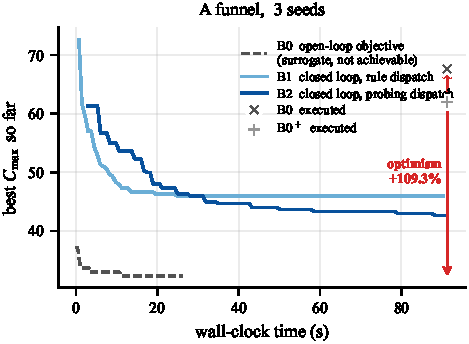
\includegraphics[width=\columnwidth]{fig/fig_convergence_closedloop.pdf}
\Description{Best-so-far makespan against wall-clock time for three
configurations, with the two-stage curve marked as a surrogate objective and its
true repaired value shown as a separate point.}
\caption{Convergence on one \texttt{high}-congestion instance, median over five
seeds under a shared $46.3$\,s budget. The two-stage curve is plotted against
its own surrogate objective, which is what it optimizes; the star marks the true
makespan after its frozen decisions are routed conflict-free. Within the same
budget two-stage completes about $1{,}980$ generations and the full closed loop
$47$.}
\label{fig:convergence}
\end{figure}

\paragraph{Nothing built on top of it pays.}
The second reading is the one we did not expect. Among the configurations that
already evaluate the true objective, quality does not improve with
sophistication---it declines. The cheapest of them is the best, and the ordering
of Table~\ref{tab:main} is close to monotone in cost: $+7.69\%$ at
$1.99$\,ms per evaluation, $+5.52\%$ at $15.37$\,ms, and $-2.80\%$ at
$77.91$\,ms, where the most elaborate configuration has fallen behind the
baseline it was built to improve on. Because the budget is fixed, every
millisecond a mechanism adds to an evaluation is a millisecond taken from the
number of evaluations, and none of the mechanisms we added returns more than it
costs. Table~\ref{tab:ablation} makes this precise one factor at a time.

\begin{table}[t]
\caption{Attribution of each mechanism, from pairs of configurations differing
in that mechanism alone. Positive means the mechanism repays its cost under an
equal wall-clock budget. ``Cost'' is the resulting multiple in ms per
evaluation. Each mechanism is switched on in two contexts; agreement between
the two rows is what makes the estimate trustworthy.}
\label{tab:ablation}
\small
%% generated by tab/gen_tables.py -- do not edit by hand
\begin{tabular}{@{}llrrcr@{}}
\toprule
Mechanism & Context & Cost & $\Delta C_{\max}$ (\%) & W/L/T & $p$ \\
\midrule
Conflict-free routing in the loop & cheap dispatch & $5.1\times$ & $+7.69^{***}$ & 138/17/5 & $<10^{-4}$ \\
 & exact dispatch & $23.7\times$ & $+6.95^{***}$ & 130/24/6 & $<10^{-4}$ \\
\addlinespace
Reservation-aware dispatch & no local search & $4.7\times$ & $-0.93^{*}$ & 60/80/20 & 0.046 \\
 & with local search & $4.9\times$ & $-0.74$ & 72/70/18 & 0.354 \\
\addlinespace
Contention-guided local search & cheap dispatch & $1.6\times$ & $-1.96^{***}$ & 53/96/11 & $1\times10^{-4}$ \\
 & exact dispatch & $1.7\times$ & $-1.72^{*}$ & 62/79/19 & 0.010 \\
\addlinespace
Staggering operator & on top of reassignment & $1.1\times$ & $-0.16$ & 66/61/33 & 0.537 \\
\addlinespace
Priced routing & on top of the full loop & $5.1\times$ & $-8.99^{***}$ & 5/143/12 & $<10^{-4}$ \\
\bottomrule
\end{tabular}

\end{table}

Read down the table, one mechanism repays its cost and three do not. Putting
conflict-free routing inside the evaluation loop costs $5.1\times$ more per
evaluation in the cheap-dispatch context and returns $+7.69\%$; in the
expensive-dispatch context it costs $23.7\times$ and still returns $+6.95\%$.
Probing the reservation table when dispatching costs a further $4.7\times$ and
returns $-0.93\%$. The contention-guided neighbourhood costs $1.6$--$1.7\times$
and returns $-1.96\%$ and $-1.72\%$. Pricing costs $5.1\times$ and returns
$-8.99\%$. The two estimates for each mechanism agree in sign and, to within a
quarter of a percentage point, in magnitude, so none of these readings depends
on the context in which the mechanism was switched on.

That agreement is worth dwelling on, because the confounded version of the same
comparison reverses the conclusion. Contrasting the proposed method with the
configuration that adds reservation-aware dispatch \emph{and} local search at
once yields $+0.83\%$ in favour of the richer configuration, at $p=0.047$: a
significant result, with the wrong sign, obtained from the same runs. The two
factors happen to push in opposite directions, and a chain-style ablation that
moves both at once reports their sum as though it were an attribution. We report
the confounded number because we believed it for some time.

Fig.~\ref{fig:ablation} shows the same comparisons per instance family,
normalized by each instance's lower bound so that cells with different bounds
share an axis.

\begin{figure}[t]
\centering
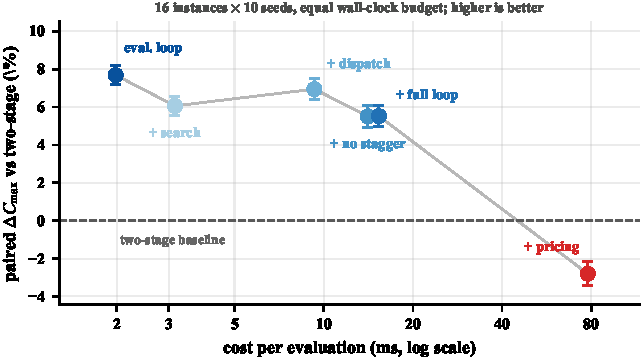
\includegraphics[width=\columnwidth]{fig/fig_ablation.pdf}
\Description{Dot plot of makespan divided by lower bound for each
configuration, separately for high and funnel congestion.}
\caption{The configurations under an equal wall-clock budget, as a ratio to the
composite lower bound (lower is better). Error bars span heterogeneity levels.
The separation between two-stage and the rest is present in every congestion
family; the separation \emph{within} the rest is not.}
\label{fig:ablation}
\end{figure}

Fig.~\ref{fig:protocol} substantiates the protocol argument of
Section~\ref{sec:protocol} rather than the method: the left panel is why equal
generations would be indefensible, and the right panel is why equal time is not
a free choice either.

\begin{figure}[t]
\centering
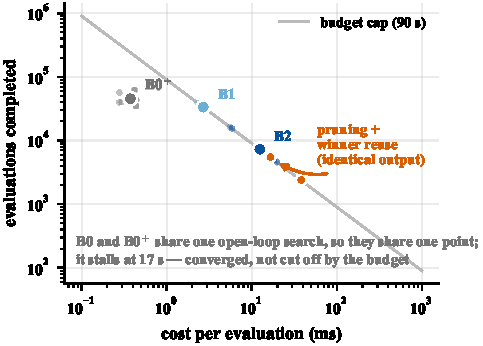
\includegraphics[width=\columnwidth]{fig/fig_protocol.pdf}
\Description{Two bar charts on logarithmic axes: cost per evaluation by
configuration, and evaluations completed within the shared budget.}
\caption{Neither budget is neutral. Evaluation cost spans a factor of $199$
across the configurations (left), so at equal wall-clock the cheaper ones
complete far more search (right). Both quantities are reported for every cell.}
\label{fig:protocol}
\end{figure}

The dependence runs deep enough to change what the paper would have concluded.
Fig.~\ref{fig:protocols} repeats four comparisons under both conventions. Equal
generations charges nothing for a local-search neighbour or a dispatch probe, and
under it the mechanism-rich configuration gains against every cheaper one---by
$2.9\%$ against rule-based dispatch, significantly, where equal wall-clock
records exactly $0.0\%$. The pricing comparison behaves the same way and more
starkly: indistinguishable from unpriced under equal evaluations, worse by $6$ to
$8\%$ under equal wall-clock (Section~\ref{sec:pricing}). Neither convention is
wrong. Equal generations answers whether a mechanism improves a search step, and
equal wall-clock answers whether it improves a search; the first is a question
about mechanism design and the second about whether to deploy it. What is not
defensible is reporting one and describing it as the other.

\begin{figure}[t]
\centering
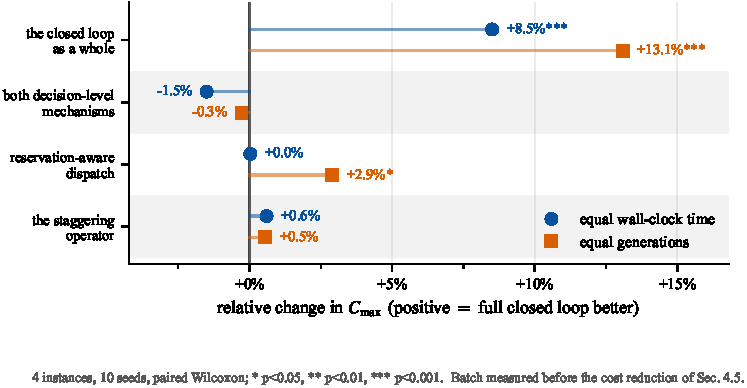
\includegraphics[width=\columnwidth]{fig/fig_protocols.pdf}
\Description{Four paired comparisons, each shown twice: once under an equal
wall-clock budget and once under an equal number of generations, with the
equal-generation reading systematically more favourable to the elaborate
configuration.}
\caption{The same four comparisons under both budget conventions, against the
full closed loop. Equal generations does not charge for the extra work a
mechanism performs, and systematically flatters it; the gap between the two
markers in a row is the part of the apparent gain that is an accounting artefact.
Measured on the four instances for which both protocols were run.}
\label{fig:protocols}
\end{figure}

\subsection{Which congestion is worth feeding back?}
\label{sec:whichcongestion}

This was intended as the sharpest test available to us, because \texttt{high}
and \texttt{funnel} differ in one controlled respect. If the mechanisms work by
steering decisions away from contention, their advantage must persist where
contention is avoidable and vanish where it is not. A mechanism that improved
both equally would be improving something else. The prediction is
falsifiable, and Section~\ref{sec:main} has already removed its subject: there
is no mechanism gain to localize. What remains testable is whether the gain of
the evaluation loop itself depends on congestion structure, and the answer is
that it does not.

\begin{figure}[t]
\centering
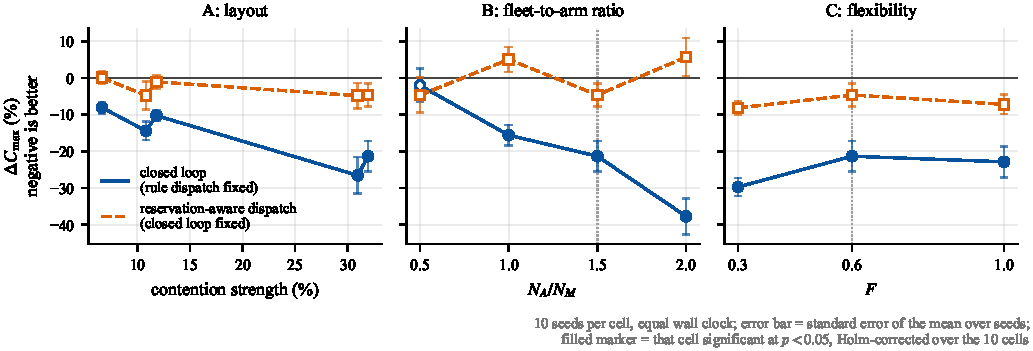
\includegraphics[width=\columnwidth]{fig/fig_prediction3.pdf}
\Description{Grouped bars comparing the gain of each mechanism under high and
funnel congestion.}
\caption{Gains under avoidable (\texttt{high}) and unavoidable
(\texttt{funnel}) congestion, paired by $(H,\text{seed})$. The two instance
families differ only in the width of the station cut.}
\label{fig:prediction3}
\end{figure}

Table~\ref{tab:bytag} gives the gain of the proposed method over two-stage in
all sixteen cells. It is large and significant everywhere, and it is not ordered
by congestion: $+8.76\%$ on \texttt{low}, $+4.03\%$ on \texttt{mid},
$+9.50\%$ on \texttt{high} and $+8.47\%$ on \texttt{funnel}. The controlled
pair is the informative one, since \texttt{high} and \texttt{funnel} differ only
in the width of the station cut: the gain falls from $9.50\%$ to $8.47\%$, a
difference far smaller than the spread across heterogeneity levels within either
family. Rank correlation between the gain and heterogeneity is $-0.21$ over the
sixteen cells, that is, slightly negative where the design predicted positive.

\begin{table}[t]
\caption{Gain of the proposed method over two-stage in every cell, by congestion
family and heterogeneity, and pooled per family ($n=40$ seed-paired comparisons
per family). Positive favours the proposed method.}
\label{tab:bytag}
\small
%% generated by tab/gen_tables.py -- do not edit by hand
\begin{tabular}{@{}lccccc@{}}
\toprule
& \multicolumn{4}{c}{$\Delta C_{\max}$ (\%) at $H=$} & pooled \\
\cmidrule(lr){2-5}
Structure & $0$ & $0.15$ & $0.3$ & $0.5$ & (\%) \\
\midrule
\texttt{low} & $+10.3$ & $+5.6$ & $+8.8$ & $+10.4$ & $+8.76^{***}$ \\
\texttt{mid} & $+3.3$ & $+4.0$ & $+4.5$ & $+4.3$ & $+4.03^{***}$ \\
\texttt{high} & $+11.3$ & $+8.1$ & $+10.7$ & $+7.9$ & $+9.50^{***}$ \\
\texttt{funnel} & $+9.2$ & $+8.7$ & $+9.4$ & $+6.5$ & $+8.47^{***}$ \\
\bottomrule
\end{tabular}

\end{table}

The reason is visible once the mechanism attributions are in hand. Our
prediction was about mechanisms that steer decisions away from contention, and
such a mechanism must indeed depend on the contention being avoidable. But the
effect that survives is not of that kind. Replacing a surrogate objective with
the true one does not steer anything; it removes a systematic bias from every
fitness value the search sees, and a bias is worth removing whether or not the
delay it hides could have been avoided. On \texttt{funnel} the unavoidable
corridor inflates every candidate's makespan, so the surrogate misranks
candidates there as badly as anywhere else. What congestion structure would
govern is the size of the \emph{mechanism} gain, and there is none to govern.

The practical reading is therefore simpler than the one we set out to make, and
less contingent: evaluate under the true routing model whatever the layout, and
do not expect a contention-aware neighbourhood to add to it. It also resolves a
discrepancy we would otherwise have had to leave open. An earlier hand-built
congested instance showed no advantage for the elaborate configuration;
measuring its structure afterwards revealed a binding funnel bound, and we
concluded at the time that the mechanisms were being asked to act on a signal
the instance did not contain. The wider matrix shows that the instance was not
special: the mechanisms do not pay on any of the four families.

\subsection{Sensitivity to heterogeneity}
\label{sec:hetero}

Reassignment trades processing time for proximity, so it needs the two to
differ. At $H=0$ all eligible arms take the same time and the trade-off is
empty; the operator can still move an operation to a less congested arm, but it
buys nothing in duration and the resulting choice is arbitrary. The design
therefore predicts that the reassignment operator becomes useful as $H$ grows,
and that its gain should be near zero at $H=0$.

\begin{figure}[t]
\centering
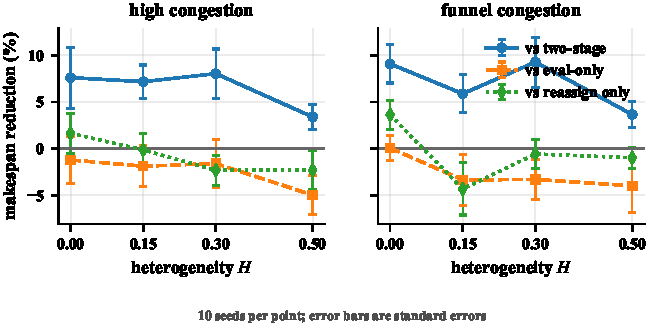
\includegraphics[width=\columnwidth]{fig/fig_heterogeneity.pdf}
\Description{Gain against heterogeneity level for each baseline, under high and
funnel congestion.}
\caption{Gain against heterogeneity. The mechanisms depend on arms differing in
speed, which is what makes ``reassign to a slower but better-connected arm'' a
decision rather than a coin flip.}
\label{fig:hetero}
\end{figure}

The prediction is not borne out, and the reason is the same as in
Section~\ref{sec:whichcongestion}: the operator has no gain at any $H$, so there
is no trend for $H$ to modulate. Contention-guided search costs $1.72\%$ at
$H=0$ and does not become profitable at $H=0.5$. The gain of the evaluation loop
is likewise flat in $H$ (Table~\ref{tab:bytag}), which is what one expects of a
correction to the objective rather than to a decision rule.

We keep this analysis in the paper because the negative form of the prediction is
still informative. Heterogeneity was our reason for believing the reassignment
operator had something to work with: an eligible set whose members differ in
speed is exactly the condition under which ``move to a slower but
better-connected arm'' is a real decision. That condition holds in these
instances by construction, and the operator still does not pay. Its failure is
therefore not a failure of the instance family to present the trade-off; it is
that finding the trade-off by local search costs more than the trade-off is
worth at the margin, as Section~\ref{sec:whycost} argues.

\subsection{Pricing the interface: a negative result}
\label{sec:pricing}

Section~\ref{sec:interface} argued that pricing corridor occupancy double-counts
a delay the fitness already sees. The argument predicts that pricing cannot add
information; it does not by itself say what the measured penalty will be, and
separating the two turns out to matter. We sweep the coordination strength
$\theta$ under both budget conventions, holding the router's search width
constant across all $\theta$ so that pricing is not confounded with the number
of entry times the router examines.

\begin{figure}[t]
\centering
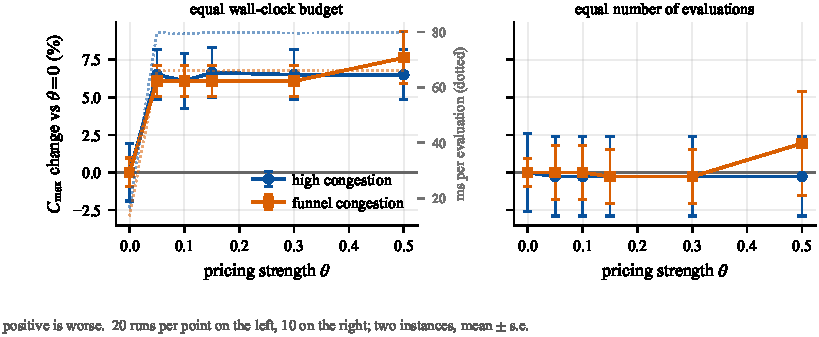
\includegraphics[width=\columnwidth]{fig/fig_theta.pdf}
\Description{Two panels of makespan change relative to theta equals zero against
pricing strength: under equal wall-clock the penalty is large and flat, under
equal evaluations it is absent.}
\caption{Pricing the interlayer interface. Positive is worse. Under an equal
wall-clock budget (left) the penalty appears the instant pricing is switched on
and is then flat over a tenfold range of $\theta$, tracking the cost per
evaluation on the right-hand axis. Under an equal number of evaluations (right)
it is absent. The harm is therefore an accounting consequence of a more
expensive route search, not evidence that the price misdirects the router.}
\label{fig:theta}
\end{figure}

Under equal wall-clock, pricing costs $6.2$ to $6.8\%$ of makespan at every
$\theta$ we tried, with $p\approx0.006$. Under equal evaluations the same
comparison yields $+0.15\%$ and $+0.28\%$---indistinguishable from zero, with
$p\ge0.75$. The explanation is in the evaluation counts: priced routing completes
$636$ to $948$ evaluations inside the budget where unpriced routing completes
$3006$ to $4500$, a factor of $4.7$. Pricing does not misrank candidates; it
starves the search.

Two further observations rule out the alternative readings. First, $\theta$ is
not a meaningful dial in this problem. Over the range $0.05$ to $5.0$---two
orders of magnitude---the priced router changes the route of the same $4$ of $24$
transport tasks, pays the same total price, and returns the same makespan. The
accumulated price amounts to $2.4\%$ of total travel time, a perturbation too
small to overturn the ordering that arrival time imposes on the scalarized
objective $\text{arrival}+\theta\cdot\text{price}$. Only at $\theta=50$ do prices
dominate arrival time, and then the makespan degrades from $75.0$ to $91.6$ on
the instance we probed: the double-counting harm does appear, but only once the
price is strong enough to override the quantity that actually determines
feasibility. Second, the cost is structural rather than a consequence of prices
being non-zero. A single decoding takes $9.0$\,ms unpriced and $45$ to $47$\,ms
priced, and that multiple is identical at every $\theta$, because it is paid for
maintaining a Pareto frontier per node and trying several entry times per arc
whether or not any price is charged. Nor can the price table be made
informative by enlarging it: raising the retained slot count from $24$ to $200$
yields the same $11$ slots, covering $11\%$ of the corridor--time cells, because
the table is limited by how few critical slots a solution has rather than by the
cap.

We report this at length because the negative result is more transferable than a
positive one would be, and because the two protocols disagree about its size but
not its sign. The theoretical argument does not depend on our price estimator:
whether prices come from a finite-difference probe of corridor capacity or from a
critical-chain surrogate, they charge for an occupancy whose consequence has
already been paid, in full, inside the arrival time of the vehicle that yielded.
Any architecture that evaluates fitness by a complete conflict-free decoding will
have this property, and the empirical form the property takes is that the price
is inert. What then decides the comparison is the cost of the machinery required
to act on an inert signal. The corollary for design is accordingly sharper than
the one we set out to draw: before enriching an interlayer interface, check
whether the receiving layer's objective already internalizes what the interface
would carry, because if it does, the enrichment is not merely unhelpful but
strictly costly.

\subsection{Why the mechanisms do not pay}
\label{sec:whycost}

The comparisons above establish that three mechanisms fail to repay their cost;
they do not explain why. Two measurements do.

The first is where the compute goes. Instrumenting the search to count
decodings separately shows that contention-guided local search consumes
$39.4\%$ of all decodings performed, and that of the neighbours it decodes,
$1.4\%$ improve the makespan through reassignment and $0.6\%$ through
staggering. Nearly two-fifths of the budget is therefore spent on a
neighbourhood in which fewer than one candidate in fifty is an improvement. The
comparison that matters is not whether those improvements are real---they
are---but whether the same decodings returned to the population loop would
produce more. At these hit rates they do, and that is the whole of the effect
measured in Table~\ref{tab:ablation}.

The low hit rate is not a defect of implementation, and we spent some effort
establishing that. The neighbourhood is small and pointed by construction, at
most $L+2=7$ candidates per round, every one named by the lower layer; a
low hit rate on a pointed neighbourhood means the certificates identify
operations whose reassignment or displacement does not shorten the critical
chain. We attempted three targeted repairs---scoring reassignment candidates by
the expected yielding along the path rather than by ideal distance, replacing
adjacent swaps with targeted insertion in the staggering operator, and admitting
plateau moves that reduce total yielding at equal makespan---and evaluated each
independently against the unmodified operator under an equal-evaluation budget.
None reached significance. We report the attempt because it bounds the
conclusion: the failure lies in the signal rather than in how we acted on it.

The second measurement is why the signal is weak. A contention certificate
names the corridor, interval and opposing task of a yielding event, which is
precisely the information needed to remove \emph{that} event. But the makespan is
attained through a chain, and removing one corridor delay usually promotes a
different constraint to binding---an upstream operation, a machine, or another
corridor---so the realized improvement is a fraction of the delay removed. Our
own acceptance rule re-extracts the chain after every accepted move for exactly
this reason. Feedback that names a bottleneck is therefore worth much less than
its magnitude suggests whenever the bottleneck is one of many comparable ones,
and the same reasoning applies to reservation-aware dispatch: probing the table
picks the vehicle that arrives soonest for the task at hand, which is a local
improvement whose effect on the makespan is diluted through the same chain.

This is what distinguishes the one mechanism that pays from the three that do
not. Conflict-free evaluation is not a better decision; it is a better
\emph{measurement}, applied to every candidate the search will ever compare. Its
benefit does not have to survive dilution through a chain, because it does not
act on the chain at all---it corrects the ranking. That asymmetry, rather than
anything specific to our operators, is what we would expect to transfer.

\subsection{Threats to validity}
\label{sec:threats}

\emph{Instance family.} All cells share one size and one layout template. The
factors we vary are the ones our analysis identifies as decisive, but size and
topology are held fixed, and we make no claim about how the mechanisms scale.

\emph{Absence of a public benchmark comparison.} The standard FJSP\_PT
benchmarks assume a constant travel matrix and provide no aisle network, so
they cannot express vehicle contention; running on them would require deleting
the constraint the paper is about. A degenerate comparison---our upper layer
against published results with routing switched off---would test the genetic
algorithm rather than the framework, and we have not performed it.

\emph{Bound quality.} The composite lower bound is loose, with gaps to the best
known solutions ranging from $34\%$ to $68\%$ for the proposed method, with a
median of $53\%$. It serves to keep the numbers honest and to catch regressions,
not to certify optimality; a gap of that size cannot distinguish a search failure
from a slack bound, and we make no claim about proximity to the optimum. Exact solutions for
small instances, which logic-based Benders decomposition has been shown to
deliver for this problem class~\cite{vanos2026exact}, would settle how much of
the remaining gap is search failure rather than model structure; we regard this
as the most valuable next step.

\emph{Single implementation.} Every arm shares one codebase, which removes
implementation variance between arms but means the absolute makespans reflect
the quality of that implementation. The ablation differences, being internal,
are unaffected; comparisons against published methods would not be.

\section{Conclusion}
\label{sec:Chapter_VI}

We studied integrated scheduling of heterogeneous robot arms and conflict-free
AGV routing under the assumption the literature usually avoids: that travel time
is produced by routing decisions rather than read from a matrix. Within that
setting we asked a narrower question than the usual one. Not whether closing the
loop between scheduling and routing helps---it does---but which of the things a
routing layer could tell a scheduler are worth what they cost, when the budget is
fixed and every answer is paid for in evaluations forgone.

\subsection{Summary of Contributions}
\label{sec:contributions}

The answer is more one-sided than we expected. Of four mechanisms implemented in a
common codebase and compared over $16$ controlled instances with $10$ seeds under
an equal wall-clock budget, exactly one repays its cost. Evaluating fitness by a
complete conflict-free decoding reduces makespan by $7.7\%$ against a two-stage
open-loop baseline, and it does so while performing five times \emph{fewer}
evaluations than that baseline, whose cheap surrogate is optimistic by $25.9\%$ on
the instance we trace. Reservation-aware dispatch, contention-guided local search
and corridor pricing all cost more than they return, by $-0.9\%$, $-1.7\%$ and
$-9.0\%$; each estimate is obtained twice, from configurations differing in that
mechanism alone, and the pairs agree to within a quarter of a percentage point.
The proposed method is therefore the cheapest configuration that evaluates the
true objective, and the paper's substantive claim is that this is not an accident
of our operators but a consequence of what the two kinds of intervention do. A
corrected objective improves the ranking of every candidate the search will
compare, at a price paid once per evaluation. A mechanism that names a bottleneck
buys a local improvement that dilutes through the critical chain, because removing
one delay promotes another constraint to binding---which is why contention-guided
search can consume $39.4\%$ of all decodings while fewer than one neighbour in
fifty improves the makespan.

Two negative results are reported in full because their mechanisms transfer
further than another heuristic would. Pricing an interlayer interface fails
whenever the receiving layer's objective already internalizes what the price would
charge for, and the failure is quantitative rather than qualitative: the price is
inert, altering $4$ of $24$ routes over a hundredfold range of pricing strength,
while the multi-label search required to read it costs five times more per
decoding whether or not any price is charged. And a comparison protocol that does
not equalize computation, or that moves two factors at once, does not merely lose
power---it produces significant results with the wrong sign. Our own chain-style
ablation reported reservation-aware dispatch as beneficial at $+0.83\%$
($p=0.047$) where the de-confounded contrast gives $-0.93\%$ ($p=0.046$) on the
same runs.

\subsection{Limitations and Future Directions}
\label{sec:future_work}

\textbf{(1) The scope of the negative results.} Our instances share one size, one
layout template and one fleet-to-arm ratio, and all four mechanisms were judged
under a budget calibrated from a pure-Python implementation. The exchange rate
between cost and evaluations is what our comparisons measure, and it is measured
between configurations sharing an implementation, so it is robust to a constant
speedup. It is not robust to a change in the \emph{relative} cost of the pieces. A
routing layer with an incremental evaluator, able to re-decode a locally perturbed
solution without replaying the whole sweep, would lower the price of exactly the
mechanisms that failed here, and the contention-guided neighbourhood is the
natural first candidate to re-test under it. We regard our results as
establishing that these mechanisms do not pay at present costs, not that they
cannot pay.

\textbf{(2) Larger and structurally different shops.} The dilution argument of
Section~\ref{sec:whycost} predicts that guidance becomes more valuable as the
critical chain becomes less substitutable---a shop with one dominant bottleneck
rather than many comparable ones. Our four congestion families were designed to
vary avoidability rather than substitutability, and the funnel share we introduced
to quantify the former turned out not to distinguish the families it was meant to
separate. An instance family parameterized by chain substitutability, and an
indicator validated against the manipulation it claims to measure, would test the
explanation rather than merely be consistent with it.

\textbf{(3) Distance from the optimum.} The composite lower bound leaves a median
gap of $53\%$, which is too loose to separate search failure from bound slackness.
Exact solutions for small instances, which logic-based Benders decomposition has
been shown to deliver for this problem class~\cite{vanos2026exact}, would settle
how much of the gap is recoverable and would also test whether the mechanisms that
fail to pay under a heuristic search remain unprofitable when the search is
stronger.

\textbf{(4) Dynamic operation.} The formulation assumes known processing times and
a fixed job set. Online arrivals and vehicle breakdowns change the calculus we
report, because a mechanism's value then includes how quickly it repairs a
schedule rather than only how well it builds one; a cheap evaluator that must
re-solve from scratch may compare differently against guidance that localizes the
damage.


%\section*{Acknowledgments}
%This work was supported partly by Key Laboratory of Computer Network and Information Integration (Southeast University) of Ministry of Education of China under Grants NO. 93K-9 and Jiangsu Provincial Key Laboratory of Network and Information Security under Grants No.BM2003201.

%%
%% The next two lines define the bibliography style to be used, and
%% the bibliography file.
\bibliographystyle{ACM-Reference-Format}
\bibliography{reference-base}


%%
%% If your work has an appendix, this is the place to put it.
\appendix



\end{document}
\endinput
%%

